% TEMPLATE for Usenix papers, specifically to meet requirements of
%  USENIX '05
% originally a template for producing IEEE-format articles using LaTeX.
%   written by Matthew Ward, CS Department, Worcester Polytechnic Institute.
% adapted by David Beazley for his excellent SWIG paper in Proceedings,
%   Tcl 96
% turned into a smartass generic template by De Clarke, with thanks to
%   both the above pioneers
% use at your own risk.  Complaints to /dev/null.
% make it two column with no page numbering, default is 10 point

% Munged by Fred Douglis <douglis@research.att.com> 10/97 to separate
% the .sty file from the LaTeX source template, so that people can
% more easily include the .sty file into an existing document.  Also
% changed to more closely follow the style guidelines as represented
% by the Word sample file. 

% Note that since 2010, USENIX does not require endnotes. If you want
% foot of page notes, don't include the endnotes package in the 
% usepackage command, below.

% This version uses the latex2e styles, not the very ancient 2.09 stuff.

% Updated July 2018: Text block size changed from 6.5" to 7"

\documentclass[letterpaper,twocolumn,10pt]{article}
\usepackage{usenix2019,epsfig,endnotes}

\usepackage{pgfplots}
\pgfplotsset{compat=newest}
\usepackage{footnote}
\makesavenoteenv{tabular}


\begin{document}

%don't want date printed
\date{}

%make title bold and 14 pt font (Latex default is non-bold, 16 pt)
\title{\Large \bf 9Back : Making Our Plans Great Again}

%for single author (just remove % characters)
\author{
{\rm Maxwell Bland}
\and
{\rm Leon Cheung}\\ \\
University of California, San Diego
\and
{\rm Kilian Pfeiffer}\\
% copy the following lines to add more authors
% \and
% {\rm Name}\\
%Name Institution
} % end author

\maketitle

% Use the following at camera-ready time to suppress page numbers.
% Comment it out when you first submit the paper for review.
\thispagestyle{empty}


\subsection*{Abstract}
The following paper describes a set of benchmarks run on the Plan 9 operating system. In particular, it uses the only actively developed branch, 9FRONT "RUN FROM ZONE!" (2018.09.09.0 Release). The goal of this project is to provide researchers and enthusiasts with greater insight into the current state of the operating system's performance and capabilities of interaction with hardware. Through tests of CPU, Memory, Network, and File System operations, we will gain insight on bottlenecks in the system's performance and the interactions between low-level (hardware) and high-level (OS) system components. These performance statistics will be contrasted with subjective experiences of ``responsiveness''.

\section{Introduction}

Plan 9 from Bell labs is a distributed operating system which emerged around the 1980's. It built upon the ideas of UNIX, but adopted an ideology that ``everything is a file''. Although the system was marketed in the 90's, it did not catch on, as prior operating systems had already gained enough of a foothold. Eventually, during the 2000's, Bell Labs ceased development on Plan 9, meaning official development halted. Unofficial\footnote{This is debatable. If you adopt an orphan, are they not your official child?} development continues on the 9front fork of the codebase, with new support for Wi-Fi, Audio, and everything anyone could ever want or need. 

The experiments were performed as a group using a shared codebase and a single machine described in the following section. The measurements were performed via programs written in Plan 9's \textit{special} version of C 99. The compiler used were the x86 versions of Plan 9's C compiler, 8c. The compiler was run with optimizations disabled. Version numbers are not available. Measurements were performed on a single machine running Plan 9 directly from hardware; given the nature of the Plan 9 system,
additional metrics could be established for networked file systems and CPU servers; these measurements were not done for sake of simplicity, and because results under these conditions should be inferrable from the results cataloged within this paper plus network overheads. 

The use of actual hardware for this task should have less variance compared to measurements performed within a VM, although there were several points in time where it became clear that Plan 9 was not neccessarily able to handle the hardware interface as expected, such as during the high contention disk access task, which caused I/O errors to shoot off from the SSD.

The project was accomplished over the course of ten weeks in short five to twenty hour bursts, wherein team members took turns on implementation tasks according to their respective amounts of free time. In total, due to difficulties inherent with the particular operating system chosen for benchmarking, each team member spent around 30 to 40 hours on this project. 

Benchmarking a forty year old bunny-focused OS maintained by less than 10 strangers including us and making it jump through rings of fire was admittedly a weird flex but okay. 

\section{Machine Description}

We ran this beautiful operating system of the gods on a Thinkpad T420, the machine of true developers.

{\tt \small
\begin{verbatim}
    Processor: model, cycle time, cache sizes (L1, L2,
      instruction, data, etc.)
      Intel(R) Core(TM) i5-2520M CPU @ 2.50GHz (Sandy Bridge)
      cache size 3072 KB
      L1$	128 KiB	
        L1I$	64 KiB	2x32 KiB	8-way set associative	 
        L1D$	64 KiB	2x32 KiB	8-way set associative	write-back
      L2$	512 KiB 2x256 KiB	8-way set associative	write-back
      L3$	3 MiB   2x1.5 MiB	12-way set associative	write-back
      cpu family 6
      model 42
      stepping 7
      siblings 4
      cores 2
      fpu yes
      fpu_exception yes
      fpu_exception yes
      bogomips 4986.98
      clflush size 64
      cache_alignment 64
    Details at https://en.wikichip.org/wiki/
    intel/core_i5/i5-520m 

    Memory bus
      DDR3-1333
      i/o-bus-frequency: 666MHz
      bus-bandwith:  10656 MB/s
      memory-clock:  166MHz
      Column Access Strobe (CAS) latency:

    I/O bus
      SataIII-speed: 600MB/s

    RAM size
      8 GB
    Disk: capacity, RPM, controller cache size
      Samsung SSD 860 EVO 500GB
      Capacity: 500GiB
      RPM: 550MB/s read, 520 MB/s write
       and 98,000 IOPS (Read QD32)
      Controller Cache Size: 512MB 
    Network card speed:
     Intel 82579 LM Gigabyte: 1Gb/s
     intel Centrino Ultimate-N 6300: 450 Mbps
      
    Operating system (including version/release) 
      9FRONT "RUN FROM ZONE!" (2018.09.09.0 Release)
\end{verbatim}
}

\section{Experiments}

For each section, we report the base hardware performance, make a guess as to how much overhead software will add to base hardware performance, combine these two into an overall prediction of performance, and then implment and perform the measurement. In all cases, we run the experiment multiple times, and calculate the standard deviation across measurements. We use the \texttt{cycles()} syscall to record the timestamp. Dynamic CPU frequency scaling was disabled for all trials, and all trials were restricted to a single core.

\subsection{Measurement Overhead (Reading Time)}

The following section reports overheads of reading time. One trial involves looping over 16 \texttt{cycles} timing calls, $2^{16}$ times. We average out for each call of \texttt{cycles}, and we do 64 trials altogether.

Since we imagine getting the current cycles clock is a fast operation, so we
estimate the hardware performance to be on the scale of nanoseconds, since one
clock cycle takes approximately 0.5 nanoseconds. We think that the
\texttt{cycles} call should do something similar to reading from the cycle
counter, so it should be almost instantaneos, perhaps on the order of 2ns.
\footnote{Page 547 of https://www.intel.com/content/dam/www/public/us/en/\\ 
documents/manuals/64-ia-32-architectures-software-developer-vol-2b-manual.pdf}

The software cost of this should be low to non-existent, since that value is 
directly loaded into two registers, which might be directly examined under normal 
circumstances. It is the case that Plan 9's C compiler does not accept assembly directives, 
and thus we were forced to use the \texttt{cycles} call, which may be doing extra work.

This would put our predicted cost at around 2 to 10 nanoseconds, accounting for potential
variations due to operating system tasks such as context switching, interrupts, and 
other architectural lags.

Our results are shown in table 1; it seems we may have underestimateed the cost of hardware 
and software in measurement of time. We feel that our methodology, however, is sound, given the
incredibly low degree of variability in our results. Units are reported in nanoseconds.

\subsection{Measurement Overhead (Loop Overhead)}

In order to measure the loop overhead, we took the time at the end of a loop
iteration and at the start of a loop iteration, and find the difference between
those to measure the loop overhead time. We repreat this 16384 times within
each trial, and perform 64 trials. We average over all of these trials.

The cost of doing a single for loop based branch in hardware is also very low.
Assuming a compare, jump, and register increment take 3 to 5 cycles, and adding
additional overheads for branch misprediction, the loop overhead should be around
10 cycles. 
\footnote{Patterson, David A.; Hennessy, John L. Computer Organization and Design: The Hardware/Software Interface.}

Software, will slow this down due to random interruptions while executing, as mentioned before.
Other system processes may need the processor, and thus the latency might be roughly twice 
this.

As a prediction, the cost of a loop will be on the order of 20 nanoseconds, maybe less, since
our hardware estimate may be a bit too lenient.

The results for this experiment are also in table 1; we did underestimate the cost of a loop by a bit;
we feel this is most likely due to higher hardware costs than expected, perhaps due to the ineffiencies
of the processor's branch predictor or just high cycle count instructions. We have every reason to believe our methodology was sound.

\begin{figure}
	\centering
    \begin{tabular}{lll}
      & Reading (ns) & Loop (ns) \\
Hardware Guess  & 1 & 5\\
Software Multiplier & 2-10 & 2 \\
Prediction & 2-10 & 10\\
Average  & 11 & 17.2 \\
Std Dev. & 0 & 0
\end{tabular}
\caption{Measurement Overheads}
\label{tab:generaloverheads}
\end{figure}


\subsection{Procedure Call Overhead}

In measuring the function overhead, we created functions of zero to seven integer arguments,
we then proceeded to call eacah of these functions 20000 times, and found the average time taken over these 20000 calls. Overall, increment overhead was almost non-existent.

The hardware cost of a procedure call using the standard c calling convention should not be that high, as it is almost all done in registers. The caller pushes the arguments to the stack (very little cost), saves the return address, the frame pointer, and calls the function. There is also all the take-down cost for the function call, and the jumping of the instruction pointer, which will clear the incoming buffer of instructions. The hardware cost of this should be significant but not insane; we
are thinking on the order of 30 cycles, so around 15 or less nsec.
\footnote{https://9p.io/sys/doc/compiler.html}

The software cost of a function call in plan 9 is remarkably small, as the compiler stores all argument positions relative to a stack pointer, and thus needs to consider only one piece of metadata while making a call. There is still the threat of context switches, so the software cost may be a multiplier between 1 and 2.

This puts our prediction for the cost to be somewhere around 15 to 20 nanoseconds for a function call, independent of the number of parameters passed.

Our results are recorded in table 2; we were roughly in line with our estimates, though there is a significant degree of variance in the results, most likely due to needing to make a reference back into DRAM or context switches. This was a straightforward quantity to measure and most likely our results are accurate. 

As a final note, there is little overhead for adding arguments to a function call in plan nine, most likely due to the stack pointer relative addressing and our lack of tests for access times to the arguments vs other operating systems.

\begin{figure}
	\centering
\begin{tabular}{lll}
Hardware Guess       & 15 nsec & \\
Software Multiplier Guess       & 1-2 &  \\
Prediction       & 17 nsec &  \\
    Num Args & Average (nsec)   & Std Dev. (nsec)  \\
0& 14.487840& 8.702724
1& 14.892560& 8.991838
2& 15.215200& 9.187626
3& 14.844640& 8.996905
4& 14.883760& 8.986072
5& 15.223920& 9.204537
6& 14.851200& 8.963965
7& 15.226480& 9.198042
8& 15.264640& 9.227006
\end{tabular}
\caption{Procedure Call Overheads}
\label{tab:proccalloverheads}
\end{figure}

\subsection{System Call Overhead}

To measure the syscall overhead, we used the \texttt{errstr(2)} syscall, in
particular, \texttt{rerrstr(char*, vlong)}. \texttt{reerrstr} reads the error
string for the error of a previous syscall, and does not clear the errstr
buffer. Within each trial, we performed the syscall 16384 times, and averaged
over 64 trials.

Data from IBM puts the cost of making a system call on the Pentium processor in 1997/1995
to be 223 cycles, or roughly 1.68 usec for that processor. Our processor is much faster,
putting the timing at around 100 nsec.
\footnote{https://www.ibm.com/developerworks/community/blogs/kevgrig/entry 
/approximate\_overhead\_of\_system\_ calls9?lang=en}

It is likely that the overhead of a syscall beyond this is pretty high due to
the actual operations and implementation of the syscall operation. Thus, the
cost could be 10x the hardware cost.

That puts our estimate at around 1000 nsec or 1usec, which still seems reasonable for a system call.

Results are shown in table three and reveal a slight overestimate on our part, though perhaps not an 
unreasonable one. Notably, this cost is much, much higher than a empty-body procedure call. We do not
have any reason to believe that Plan 9 would be caching the results of this system call so that subsequent
calls do not need to trap to the OS. This may be a potential source of optimizations.

Our methodology for evaluating this experiment was straight forward enough and is likely correct.

\begin{figure}
	\centering
    \begin{tabular}{ll}
            & System Call Overhead \\
    Hardware Guess  & 100 nsec  \\
    Software Multiplier  & 10x \\  
    Prediction  & 1000 nsec \\
    Average  & 861 nsec\\
    Std Dev. & 70.8 nsec          
    \end{tabular}
\caption{Syscall Overhead}
\label{tab:syscalloverheads}
\end{figure}

\subsection{Task Creation Time}

We measured process creation overhead in two different ways, one in which we
\texttt{rfork}'ed a new process without copying the parent state to the child,
and, \texttt{fork}, where the child will copy all of the parent's file
descriptors, and share the other state as normal. We do these 20000 times for
each type of \texttt{fork} and we average over all of these calls. This methodology
results from the fact that Plan 9 does not have kernel threads.

The hardware costs of a light fork should be much less than a heavy fork, since
resources do not need to be shared, but because our processes are minimal, it
is likely this difference is negligible. Plan 9 adopts a very similar memory management
scheme to Unix, and so fork semantics are roughly equivalent, including copy-on-write. (The 
following citation contains a breakdown of almost every line in the Plan 9 kernel source code).
\footnote{http://citeseerx.ist.psu.edu/viewdoc/download? doi=10.1.1.75.5409\&rep=rep1\&type=pdf}. The number
of cycles involved in forking a process is likely huge, however, and in the tens of thousands of 
cycles, since all sorts of meta data (such as the page table) needs to be copied over. There 
aren't many good resources online which have benchmarked the number of cycles involved in a fork.

Since the software overhead of a fork is the fork itself, the hardware and software costs are 
pretty much interlinked in this particular experiment. Thus, we ignore a software multiplier, setting it
equal to 1. 

That puts our estimate at around 60,000 cycles or 30,000 nsec for both fork operations. We do not 
believe that Plan 9's lightweight fork operation will help much, and that most of the resources 
and state will still need to be copied to the child.

Our results are recorded in table 4; we were roughly in line with our estimates, but there is something quite interesting going on with Plan 9's heavy fork, the equivalent of running a process vs. a kernel thread. There is no difference in average fork time, but there is a huge variation in the two. Heavy forks have a long tail; in future work, it may be interesting to plot this long tail, and analyze the impact it has on end-user applications.

In general, programmers should opt for light forks, if possible. Just don't bend them!

\begin{figure}
	\centering
\begin{tabular}{lll}
        & Light Fork & Heavy Fork \\
Hardware Guess & 30 usec & 30 usec \\
Software Multiplier & 1x & 1x \\
Prediction & 30 usec & 30 usec \\
Average & 27.250  usec & 28.674  usec \\
Std Dev & 1.83 usec & 58.068 usec                  
\end{tabular}
\caption{Fork Overheads}
\label{tab:forkoverheads}
\end{figure}

\subsection{Context Switch Time}

Finally, to measure context switching, we created a pipe in a parent process,
and forked off a new child process. We forced a context switch by writing to
the pipe in the parent and then waiting for the child to read from the pipe
and terminate. We take the time between when the parent goes to sleep and when
the parent wakes up again after the child's termination. Then, we subtract
the overhead of reading from the pipe and closing the pipe (which happens in
the child), and divide the time in half to account for the two context switches.
We repeat this measurement 1000 times and use a new pipe each time. To take
the time of a context switch, we take the minimum time over all of these trials.

We estimated the base hardware cost of context switching while pinned to a single CPU to
be on the order of around 1600 ns based upon benchmarks done on the Intel E5-2620, another
Sandy Bridge processor model. \footnote{https://blog.tsunanet.net/2010/11/how-long-does-it-take-to-make-context.html}

Our prediction for the software cost of this is going to be quite large, most likely around 10x, since there
are so many factors involved and our method of triggering a context switch is not the most scientific 
method due to limitations in low-level threading primitives for Plan 9. 

This puts our prediction right around 16 usec; the cost of the context switch itself may be less than 
this in Plan 9, but in order to measure this, we will need to develop modifications to the kernel. 
These modifications are reserved for future work.

The results are included in table 5. Our estimates were a bit too pessimistic, however, they were close 
to the truth, as the results were skewed to values even greater than 16 microseconds. 

In general, our methodology could be improved; a lack of familiarity with such a niche system reduced our ability to benchmark effectively. 

\begin{figure}
	\centering
\begin{tabular}{ll}
Hardware Cost  & 1600 nsec  \\
Software Multiplier  & 10x   \\
Prediction  & 16 usec    \\
Average  & 13.458 usec    \\
Std Dev. & 9.569 usec     \\
Min      & 7.862 usec   
\end{tabular}
\caption{Context Switch Overheads}
\label{tab:conswitchoverheads}
\end{figure}

\subsection{RAM Access Time}

To measure ram access time we allocate a $1.6$ GB array on the heap, and iterated through it with changing stride size to hit L1, L2 cache and finally memory. The stride size gets increased by factor 1.01 for each iteration. Predictions are presented in fig.~\ref{tab:accesstimepred}, while the measurements are presented in fig.~\ref{tab:accesstime}. Figure~\ref{fig:memlatency} presents the plot of the mean in orange and standard deviation in blue with the last index accessed in the iteration on the $x$ axis, and memory access latency is displayed on a logarithmic scale $y$ axis. The measurements are not completely free of overhead, but still a transition from L1 to L2, and from L2 to memory is visible in the graph. 

We estimated the base hardware cost of memory accesses based upon well documented knowledge of the timings of such memory accesses. According to work done on breaking AES, L1 cach is available after 3 cycles, L2 after 11, and memory after this takes hundreds of cycles. 
\footnote{http://palms.ee.princeton.edu/system/files/Cache-timing+attacks+
on+AES.pdf}

For measurements like the one outlined above, there is very little software cost involved; thus our software overhead estimate is a multiplier of 1.

As a result, our prediction is that the memory access times under Plan 9 will correspond well with other 
operating systems and personal computers, particularly those running x86 processors.

And our results, shown in tables 6, 7, and figure 8, reveal that our prediction was, indeed, correct. Standard deviations were high for some portions, due to natural variations in experimental conditions. This is an 
important result from a security point of view, as it reveals that Plan 9 may be vulnerable to significant 
timing side channel attacks, something which should be addressed by the community in due time, especially
considering the distributed nature of the Plan 9 system.

Our methodology has revealed a common expectation and typical empirical feature of x86 processors, and 
thus we are confident in our methodology.

\begin{figure}
	\centering
	
	\begin{tabular}{lll}
		prediction L1 latency  & 2-3 cycles & 0.8-1.2 nsec  \\
		prediction L2 latency  & 10 cycles  & 4 nsec \\
		prediction memory latency  & 100 cycles   & 40 nsec \\
	\end{tabular}
	\caption{RAM access time prediction}
	\label{tab:accesstimepred}
\end{figure}

\begin{figure}
	\centering

	\begin{tabular}{ll}
		L1 latency  & 6 nsec  \\
		L2 latency  & 10 nsec  \\
		Memory   & 250 nsec   \\
	\end{tabular}
	\caption{RAM access time measurements}
	\label{tab:accesstime}
\end{figure}

\begin{figure}
	\centering
	% This file was created by matplotlib2tikz v0.6.18.
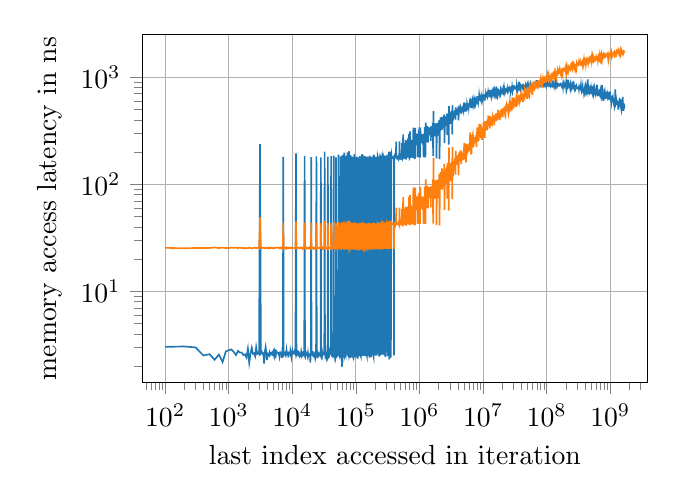
\begin{tikzpicture}

\definecolor{color0}{rgb}{0.12156862745098,0.466666666666667,0.705882352941177}
\definecolor{color1}{rgb}{1,0.498039215686275,0.0549019607843137}

\begin{axis}[
height=6cm,
tick align=outside,
tick pos=left,
width=8cm,
x grid style={white!69.01960784313725!black},
xlabel={last index accessed in iteration},
xmajorgrids,
xmin=43.5293709083906, xmax=3850966979.34791,
xmode=log,
y grid style={white!69.01960784313725!black},
ylabel={memory access latency in ns},
ymajorgrids,
ymin=1.40359602278608, ymax=2497.90842974935,
ymode=log
]
\addplot [semithick, color0, forget plot]
table [row sep=\\]{%
100	3.0246348 \\
200	3.0494168 \\
300	2.990374 \\
400	2.516836 \\
500	2.5826992 \\
600	2.2903484 \\
700	2.5637472 \\
800	2.1818744 \\
900	2.7439416 \\
1000	2.8114052 \\
1100	2.8621672 \\
1200	2.704142 \\
1300	2.5348264 \\
1400	2.7712812 \\
1500	2.6713292 \\
1600	2.6759252 \\
1700	2.5348768 \\
1800	2.5761492 \\
1900	2.4129784 \\
2000	2.912 \\
2100	2.1463868 \\
2200	2.6165748 \\
2300	2.9663068 \\
2400	2.6131972 \\
2500	2.6397092 \\
2600	2.4734884 \\
2700	3.0006292 \\
2800	2.608736 \\
2900	2.672096 \\
3000	2.594764 \\
3100	236.7831108 \\
3200	2.647456 \\
3300	2.7282696 \\
3400	2.6104528 \\
3500	2.6327172 \\
3600	2.1095744 \\
3700	2.7207528 \\
3800	3.008 \\
3900	2.6644204 \\
4000	2.2731264 \\
4100	2.6230244 \\
4200	2.5979192 \\
4300	2.5219168 \\
4400	2.6904276 \\
4500	2.5705284 \\
4600	2.6484712 \\
4700	2.6686444 \\
4800	2.5529404 \\
4900	2.5404756 \\
5000	2.7082572 \\
5100	2.5637472 \\
5200	2.7143 \\
5300	2.4895816 \\
5400	2.647456 \\
5500	2.5467656 \\
5600	2.7569724 \\
5700	2.7145356 \\
5800	2.6629308 \\
5900	2.6571084 \\
6000	2.6605744 \\
6100	2.5791284 \\
6200	2.6191176 \\
6300	2.4383076 \\
6400	2.5589496 \\
6500	2.6385936 \\
6600	2.5896284 \\
6700	2.5996924 \\
6800	2.59432 \\
6900	2.3820124 \\
7000	3.0198912 \\
7100	2.6493892 \\
7200	180.0942052 \\
7300	2.516582 \\
7400	2.54249 \\
7500	2.5725192 \\
7600	2.6356812 \\
7700	2.6609592 \\
7800	2.5826992 \\
7900	2.5194792 \\
8000	2.598264 \\
8100	2.778846 \\
8200	2.5848792 \\
8300	2.5711756 \\
8400	2.6389816 \\
8500	2.6609592 \\
8600	2.5401228 \\
8700	2.6046112 \\
8800	2.56 \\
8900	2.6453764 \\
9000	2.647698 \\
9100	2.5836408 \\
9200	2.5757516 \\
9300	2.746972 \\
9400	2.6292632 \\
9500	2.6946584 \\
9600	2.6956084 \\
9700	2.5188696 \\
9800	2.6540716 \\
9900	2.6991672 \\
10000	2.7851032 \\
10200	2.602448 \\
10400	2.6202412 \\
10600	2.6358272 \\
10800	2.734596 \\
11000	2.6033824 \\
11200	2.5537924 \\
11400	194.5869612 \\
11600	2.5602 \\
11800	2.6358272 \\
12000	2.60638 \\
12200	2.5637472 \\
12400	2.7310832 \\
12600	2.7124128 \\
12800	2.6453764 \\
13000	2.509502 \\
13200	2.5669404 \\
13400	2.6008736 \\
13600	2.529822 \\
13800	2.7293956 \\
14000	2.6006276 \\
14200	2.7031952 \\
14400	2.7013004 \\
14600	2.698788 \\
14800	2.5348768 \\
15000	2.5788804 \\
15200	2.6713292 \\
15400	2.6033824 \\
15600	184.4005232 \\
15800	2.591012 \\
16000	2.522678 \\
16200	2.752 \\
16400	2.5801208 \\
16600	2.5969336 \\
16800	2.5328056 \\
17000	2.5307832 \\
17200	2.5689344 \\
17400	2.4846924 \\
17600	2.6339324 \\
17800	2.496 \\
18000	2.5689344 \\
18200	2.5811128 \\
18400	2.5801208 \\
18600	2.5699804 \\
18800	2.5125096 \\
19000	2.5234896 \\
19200	2.1596444 \\
19400	2.7218348 \\
19600	2.8295584 \\
19800	179.435396 \\
20000	2.9052668 \\
20300	2.5808648 \\
20600	2.5449056 \\
20900	2.6093248 \\
21200	2.5209016 \\
21500	2.5194792 \\
21800	2.4825792 \\
22100	2.6260968 \\
22400	2.5880464 \\
22700	2.5178532 \\
23000	2.3694592 \\
23300	2.4546316 \\
23600	2.5868096 \\
23900	181.688524 \\
24200	2.5449556 \\
24500	2.7270968 \\
24800	2.5661924 \\
25100	2.6389816 \\
25400	2.5637972 \\
25700	2.483868 \\
26000	2.516836 \\
26300	2.5883924 \\
26600	2.5657936 \\
26900	2.5565476 \\
27200	2.5307832 \\
27500	2.6628828 \\
27800	2.602202 \\
28100	178.3295108 \\
28400	2.6397092 \\
28700	2.478916 \\
29000	2.5368452 \\
29300	2.4792772 \\
29600	2.6282892 \\
29900	2.526734 \\
30200	2.5602 \\
30600	2.5784832 \\
31000	2.6415028 \\
31400	2.6916168 \\
31800	2.6617768 \\
32200	201.2484552 \\
32600	2.6873808 \\
33000	2.4879356 \\
33400	2.5336644 \\
33800	2.5637472 \\
34200	2.4431324 \\
34600	2.547168 \\
35000	2.4610372 \\
35400	2.594764 \\
35800	2.7349704 \\
36200	181.3687508 \\
36600	2.6229756 \\
37000	2.7086352 \\
37400	2.5491772 \\
37800	2.6132464 \\
38200	2.5627984 \\
38600	2.7028164 \\
39000	2.621804 \\
39400	2.6617768 \\
39800	2.59037 \\
40200	2.5883924 \\
40700	182.79463 \\
41200	2.7902 \\
41700	2.59037 \\
42200	2.4755572 \\
42700	2.4587996 \\
43200	2.664084 \\
43700	2.6520936 \\
44200	2.6292632 \\
44700	185.3309628 \\
45200	2.6152048 \\
45700	2.6663412 \\
46200	2.5411304 \\
46700	2.72 \\
47200	2.6319392 \\
47700	2.4714176 \\
48200	2.602202 \\
48700	178.1824504 \\
49200	2.5985104 \\
49700	2.516582 \\
50200	2.4710032 \\
50800	2.5022996 \\
51400	2.5836408 \\
52000	2.5557964 \\
52600	2.543698 \\
53200	189.4943272 \\
53800	2.7154784 \\
54400	2.6260968 \\
55000	2.6484712 \\
55600	2.526734 \\
56200	2.5935304 \\
56800	2.610698 \\
57400	182.4684784 \\
58000	2.6163304 \\
58600	2.4685672 \\
59200	2.5219168 \\
59800	2.50598 \\
60400	1.9723528 \\
61100	187.5918572 \\
61800	2.6195084 \\
62500	2.5457604 \\
63200	2.5125096 \\
63900	2.6195084 \\
64600	2.5234896 \\
65300	197.1481148 \\
66000	2.46893 \\
66700	2.5303788 \\
67400	2.7310832 \\
68100	2.591012 \\
68800	2.5428928 \\
69500	184.0854584 \\
70200	2.7044732 \\
71000	2.7327232 \\
71800	2.736842 \\
72600	2.5737632 \\
73400	198.7350532 \\
74200	2.4792772 \\
75000	2.5587996 \\
75800	2.5133244 \\
76600	2.483868 \\
77400	2.79904 \\
78200	203.9780576 \\
79000	2.588788 \\
79800	2.655036 \\
80600	2.6296036 \\
81500	2.387112 \\
82400	186.628244 \\
83300	2.4106432 \\
84200	2.6490028 \\
85100	2.6513212 \\
86000	181.545792 \\
86900	2.71807 \\
87800	2.5649952 \\
88700	2.5133756 \\
89600	2.6617288 \\
90500	181.0454088 \\
91500	2.6144216 \\
92500	2.4401444 \\
93500	2.5080224 \\
94500	192.541652 \\
95500	2.5711756 \\
96500	2.5551956 \\
97500	2.5247576 \\
98500	179.4947712 \\
99500	2.6904276 \\
100500	2.6470692 \\
101600	2.5966872 \\
102700	181.3945172 \\
103800	2.6835676 \\
104900	2.4527012 \\
106000	2.432 \\
107100	177.0886152 \\
108200	2.6200948 \\
109300	2.5737132 \\
110400	2.6409212 \\
111600	177.8814712 \\
112800	2.6942784 \\
114000	2.476436 \\
115200	182.648964 \\
116400	2.554544 \\
117600	2.5451568 \\
118800	2.4970256 \\
120000	180.2716892 \\
121300	2.5966872 \\
122600	2.484074 \\
123900	191.4282228 \\
125200	2.5771428 \\
126500	2.4877812 \\
127800	188.4073856 \\
129100	2.5589496 \\
130400	2.484074 \\
131800	180.1177896 \\
133200	2.56 \\
134600	2.6656212 \\
136000	183.1701524 \\
137400	2.5330584 \\
138800	2.656 \\
140200	180.6211504 \\
141700	2.483404 \\
143200	2.6178952 \\
144700	179.8238248 \\
146200	2.6144216 \\
147700	2.5428928 \\
149200	179.4785684 \\
150700	2.5717728 \\
152300	180.615282 \\
153900	2.7198116 \\
155500	2.4908664 \\
157100	180.453022 \\
158700	2.5788804 \\
160300	180.9178312 \\
162000	2.6341268 \\
163700	2.4053276 \\
165400	184.7821984 \\
167100	2.4211864 \\
168800	178.3814708 \\
170500	2.6100604 \\
172300	2.42884 \\
174100	179.9877516 \\
175900	2.5876508 \\
177700	177.90955 \\
179500	2.6131972 \\
181300	176.79276 \\
183200	2.5649952 \\
185100	181.2418608 \\
187000	2.52496 \\
188900	2.4587996 \\
190800	188.584354 \\
192800	2.607362 \\
194800	185.0523028 \\
196800	2.8178176 \\
198800	175.0395612 \\
200800	2.533614 \\
202900	176.78141 \\
205000	2.49928 \\
207100	179.8222588 \\
209200	2.5404756 \\
211300	179.8432852 \\
213500	2.5148008 \\
215700	178.4088996 \\
217900	2.6418904 \\
220100	181.7394712 \\
222400	177.2738628 \\
224700	2.6540716 \\
227000	179.03994 \\
229300	2.512102 \\
231600	178.856674 \\
234000	2.4485228 \\
236400	180.7983832 \\
238800	2.5549452 \\
241200	183.3360536 \\
243700	181.577832 \\
246200	2.5350788 \\
248700	180.4605516 \\
251200	2.8411152 \\
253800	181.7279544 \\
256400	181.7494392 \\
259000	2.5721712 \\
261600	179.6438676 \\
264300	176.5062508 \\
267000	2.5541936 \\
269700	181.2692496 \\
272400	176.954314 \\
275200	2.5777384 \\
278000	181.7297156 \\
280800	180.7885836 \\
283700	2.5015324 \\
286600	179.0383348 \\
289500	178.8756172 \\
292400	2.4414552 \\
295400	181.2620644 \\
298400	182.0539108 \\
301400	176.97945 \\
304500	2.7469256 \\
307600	180.6265184 \\
310700	174.5870932 \\
313900	174.5869092 \\
317100	2.493948 \\
320300	177.1319496 \\
323600	174.5919084 \\
326900	175.2216176 \\
330200	201.6403412 \\
333600	2.3075528 \\
337000	178.7206868 \\
340400	178.3982488 \\
343900	179.532602 \\
347400	184.9318568 \\
350900	178.8971232 \\
354500	2.39952 \\
358100	179.1801496 \\
361700	187.7798028 \\
365400	176.6564224 \\
369100	177.609354 \\
372800	175.5592328 \\
376600	176.030444 \\
380400	177.2983924 \\
384300	176.2098668 \\
388200	178.0854656 \\
392100	175.8755772 \\
396100	2.5137828 \\
400100	177.2749016 \\
404200	181.7524956 \\
408300	176.9694168 \\
412400	177.132082 \\
416600	190.0133784 \\
420800	175.7059972 \\
425100	185.095504 \\
429400	249.8539072 \\
433700	177.9419232 \\
438100	175.6987232 \\
442500	180.1567488 \\
447000	181.7456184 \\
451500	181.898856 \\
456100	178.5736044 \\
460700	175.0617056 \\
465400	172.6751096 \\
470100	180.9513532 \\
474900	182.8480084 \\
479700	176.0281172 \\
484500	250.984294 \\
489400	179.8463052 \\
494300	175.8634264 \\
499300	177.45569 \\
504300	178.5818368 \\
509400	175.0489876 \\
514500	176.6220456 \\
519700	176.8183816 \\
524900	174.7565348 \\
530200	242.202732 \\
535600	176.4968196 \\
541000	176.1787456 \\
546500	177.4357264 \\
552000	291.907806 \\
557600	178.742748 \\
563200	180.7875924 \\
568900	242.247072 \\
574600	178.3899368 \\
580400	178.2446276 \\
586300	176.162964 \\
592200	174.436408 \\
598200	175.5315192 \\
604200	258.0647984 \\
610300	175.5453504 \\
616500	174.6104236 \\
622700	178.0969272 \\
629000	197.6625648 \\
635300	244.5993276 \\
641700	248.9109932 \\
648200	177.157818 \\
654700	245.45457 \\
661300	181.4297028 \\
668000	240.6231796 \\
674700	189.8719904 \\
681500	294.824284 \\
688400	184.450406 \\
695300	174.415914 \\
702300	176.3473596 \\
709400	312.346364 \\
716500	245.3046428 \\
723700	179.852722 \\
731000	180.1615092 \\
738400	253.1294784 \\
745800	241.6630044 \\
753300	240.8819396 \\
760900	177.6263044 \\
768600	259.0130068 \\
776300	241.0600648 \\
784100	176.5160696 \\
792000	249.0462016 \\
800000	337.62762 \\
808100	182.08239 \\
816200	178.8807872 \\
824400	176.8224412 \\
832700	174.5899728 \\
841100	174.4530004 \\
849600	177.7638704 \\
858100	335.621658 \\
866700	240.667196 \\
875400	248.8109964 \\
884200	239.7487348 \\
893100	242.5095984 \\
902100	243.2922324 \\
911200	247.2494988 \\
920400	297.410694 \\
929700	177.9123856 \\
939000	240.2590304 \\
948400	296.657896 \\
957900	178.7268116 \\
967500	297.2171004 \\
977200	288.8937228 \\
987000	299.2064424 \\
996900	183.1742164 \\
1006900	300.150618 \\
1017000	177.1184904 \\
1027200	339.2237788 \\
1037500	295.7672924 \\
1047900	242.7324328 \\
1058400	293.07532 \\
1069000	282.5022504 \\
1079700	258.713742 \\
1090500	292.589082 \\
1101500	249.1448256 \\
1112600	244.9784156 \\
1123800	295.6712312 \\
1135100	262.1938364 \\
1146500	292.656304 \\
1158000	178.5964808 \\
1169600	292.197698 \\
1181300	240.7485344 \\
1193200	243.2833352 \\
1205200	342.2710316 \\
1217300	299.6723012 \\
1229500	178.3921584 \\
1241800	194.5030516 \\
1254300	376.7017328 \\
1266900	293.9582444 \\
1279600	298.9468876 \\
1292400	247.0511268 \\
1305400	298.2493024 \\
1318500	350.674594 \\
1331700	306.1003128 \\
1345100	304.1568316 \\
1358600	244.9871488 \\
1372200	341.9389416 \\
1386000	291.614806 \\
1399900	294.2167324 \\
1413900	300.0496252 \\
1428100	337.1870304 \\
1442400	300.048508 \\
1456900	299.698946 \\
1471500	337.2483948 \\
1486300	293.1852696 \\
1501200	254.422236 \\
1516300	338.438298 \\
1531500	337.2123692 \\
1546900	300.0233804 \\
1562400	294.637874 \\
1578100	348.9722772 \\
1593900	303.0455296 \\
1609900	374.3293236 \\
1626000	243.2791452 \\
1642300	184.3491812 \\
1658800	481.1881964 \\
1675400	287.6335552 \\
1692200	287.87484 \\
1709200	370.615146 \\
1726300	279.3555444 \\
1743600	339.3322292 \\
1761100	332.6747624 \\
1778800	340.02983 \\
1796600	321.6938572 \\
1814600	364.7773392 \\
1832800	329.886926 \\
1851200	174.04289 \\
1869800	372.3613776 \\
1888500	334.3413764 \\
1907400	363.0700892 \\
1926500	329.9501872 \\
1945800	284.0708052 \\
1965300	355.6098088 \\
1985000	360.455552 \\
2004900	383.0081604 \\
2025000	333.150684 \\
2045300	396.8266712 \\
2065800	171.6348452 \\
2086500	385.934942 \\
2107400	334.5656008 \\
2128500	420.472534 \\
2149800	336.6380268 \\
2171300	361.2190172 \\
2193100	398.3632432 \\
2215100	328.209026 \\
2237300	330.2595016 \\
2259700	426.5112064 \\
2282300	323.5608992 \\
2305200	366.7526864 \\
2328300	408.918682 \\
2351600	414.4457736 \\
2375200	368.8982328 \\
2399000	359.8975412 \\
2423000	387.0827272 \\
2447300	449.2235576 \\
2471800	242.9397952 \\
2496600	368.5014448 \\
2521600	364.939228 \\
2546900	401.8287424 \\
2572400	365.3395324 \\
2598200	429.2499132 \\
2624200	364.162244 \\
2650500	361.0272884 \\
2677100	399.5365824 \\
2703900	452.969266 \\
2731000	289.5617828 \\
2758400	459.2168612 \\
2786000	399.8113512 \\
2813900	427.6687036 \\
2842100	431.9503528 \\
2870600	235.0086728 \\
2899400	537.1619644 \\
2928400	413.9425612 \\
2957700	431.9976212 \\
2987300	431.4703988 \\
3017200	433.7333104 \\
3047400	441.793424 \\
3077900	366.9799496 \\
3108700	449.5259756 \\
3139800	456.5487052 \\
3171200	423.1288452 \\
3203000	463.4054996 \\
3235100	432.4272908 \\
3267500	292.0033244 \\
3300200	545.6815976 \\
3333300	396.3048844 \\
3366700	400.6218944 \\
3400400	428.5962176 \\
3434500	456.8185244 \\
3468900	462.5389 \\
3503600	429.3134296 \\
3538700	432.0125256 \\
3574100	456.6645556 \\
3609900	487.4753576 \\
3646000	454.7574324 \\
3682500	401.3956464 \\
3719400	520.8736048 \\
3756600	466.6540952 \\
3794200	477.4483108 \\
3832200	482.7220616 \\
3870600	487.0602352 \\
3909400	458.5725396 \\
3948500	461.3575456 \\
3988000	453.6726752 \\
4027900	480.9322212 \\
4068200	468.0115524 \\
4108900	395.2511484 \\
4150000	509.4573052 \\
4191600	503.6783176 \\
4233600	491.4670544 \\
4276000	506.1215868 \\
4318800	481.294992 \\
4362000	484.841256 \\
4405700	503.9540296 \\
4449800	482.2253512 \\
4494300	530.032448 \\
4539300	454.8786448 \\
4584700	502.9195304 \\
4630600	504.8674652 \\
4677000	512.4173888 \\
4723800	504.921064 \\
4771100	503.095204 \\
4818900	470.7451784 \\
4867100	504.0442848 \\
4915800	489.2358972 \\
4965000	531.6093112 \\
5014700	523.2276436 \\
5064900	580.1232728 \\
5115600	509.9839468 \\
5166800	477.2419908 \\
5218500	527.0798712 \\
5270700	523.8965616 \\
5323500	568.9163412 \\
5376800	476.9447328 \\
5430600	511.599476 \\
5485000	547.9949152 \\
5539900	509.8036552 \\
5595300	560.7098132 \\
5651300	541.6904808 \\
5707900	516.4734896 \\
5765000	523.2727524 \\
5822700	556.0726136 \\
5881000	559.2219992 \\
5939900	528.448804 \\
5999300	561.5331344 \\
6059300	563.8478136 \\
6119900	568.0403228 \\
6181100	534.6723944 \\
6243000	634.713566 \\
6305500	545.8657568 \\
6368600	566.1749572 \\
6432300	516.68063 \\
6496700	573.7105548 \\
6561700	513.6316392 \\
6627400	593.7916832 \\
6693700	590.665274 \\
6760700	612.9427268 \\
6828400	626.01926 \\
6896700	547.536208 \\
6965700	628.5349744 \\
7035400	548.9437712 \\
7105800	562.1904052 \\
7176900	582.7326664 \\
7248700	604.804106 \\
7321200	577.6492556 \\
7394500	614.3397812 \\
7468500	578.6477756 \\
7543200	601.167302 \\
7618700	581.6933304 \\
7694900	613.9144456 \\
7771900	615.7257388 \\
7849700	553.3002944 \\
7928200	644.6191824 \\
8007500	599.7351052 \\
8087600	663.403448 \\
8168500	613.465388 \\
8250200	575.9086096 \\
8332800	631.5575344 \\
8416200	595.2229028 \\
8500400	623.719448 \\
8585500	624.901248 \\
8671400	676.5196576 \\
8758200	645.9992668 \\
8845800	656.9268416 \\
8934300	616.0666768 \\
9023700	611.7413484 \\
9114000	680.2842684 \\
9205200	600.503442 \\
9297300	667.1296 \\
9390300	626.500494 \\
9484300	653.231712 \\
9579200	601.1772292 \\
9675000	644.2959568 \\
9771800	624.7603196 \\
9869600	660.3988468 \\
9968300	609.2993324 \\
10068000	642.931342 \\
10168700	690.4400968 \\
10270400	645.495632 \\
10373200	636.8139208 \\
10477000	666.7343572 \\
10581800	604.699602 \\
10687700	656.4948492 \\
10794600	696.0706324 \\
10902600	644.8814512 \\
11011700	689.4975636 \\
11121900	665.9136884 \\
11233200	673.9083948 \\
11345600	693.7818112 \\
11459100	702.2834116 \\
11573700	645.3435452 \\
11689500	711.2753664 \\
11806400	668.8111304 \\
11924500	683.4507464 \\
12043800	729.5705908 \\
12164300	709.0653932 \\
12286000	675.8717524 \\
12408900	672.520494 \\
12533000	722.9957232 \\
12658400	648.9760344 \\
12785000	761.0900228 \\
12912900	705.846164 \\
13042100	699.0249248 \\
13172600	687.7109748 \\
13304400	700.669886 \\
13437500	669.8284568 \\
13571900	703.5441888 \\
13707700	705.629652 \\
13844800	729.0627488 \\
13983300	700.4142812 \\
14123200	720.0487556 \\
14264500	706.9443876 \\
14407200	696.8958128 \\
14551300	731.2906896 \\
14696900	705.0157764 \\
14843900	737.6425584 \\
14992400	677.8376484 \\
15142400	725.7645952 \\
15293900	698.4085084 \\
15446900	729.073624 \\
15601400	701.0986076 \\
15757500	729.875648 \\
15915100	723.9635492 \\
16074300	703.4665928 \\
16235100	748.5028032 \\
16397500	729.2079036 \\
16561500	698.6117516 \\
16727200	735.7442468 \\
16894500	715.6038968 \\
17063500	782.4077996 \\
17234200	711.8195936 \\
17406600	733.5174612 \\
17580700	722.5204896 \\
17756600	711.9632352 \\
17934200	737.5982048 \\
18113600	732.398912 \\
18294800	701.037928 \\
18477800	722.966938 \\
18662600	748.3498836 \\
18849300	716.7963348 \\
19037800	740.9953436 \\
19228200	763.0953616 \\
19420500	746.7986348 \\
19614800	750.6551464 \\
19811000	756.1466108 \\
20009200	725.9847292 \\
20209300	738.7067752 \\
20411400	728.2733432 \\
20615600	761.7688344 \\
20821800	739.8045104 \\
21030100	755.2057656 \\
21240500	791.9211344 \\
21453000	743.827124 \\
21667600	773.549504 \\
21884300	750.9982248 \\
22103200	730.5093624 \\
22324300	751.7741 \\
22547600	744.6406352 \\
22773100	776.8845932 \\
23000900	775.7307724 \\
23231000	756.183948 \\
23463400	764.3874832 \\
23698100	757.9754508 \\
23935100	783.8965604 \\
24174500	747.9219268 \\
24416300	763.9977884 \\
24660500	746.9604816 \\
24907200	768.4702588 \\
25156300	776.0638448 \\
25407900	787.4177544 \\
25662000	756.3296052 \\
25918700	751.8609536 \\
26177900	765.2830948 \\
26439700	791.4624076 \\
26704100	786.928616 \\
26971200	743.218256 \\
27241000	780.234894 \\
27513500	772.0966944 \\
27788700	787.5101064 \\
28066600	776.5866772 \\
28347300	757.5525228 \\
28630800	810.1821268 \\
28917200	780.4329464 \\
29206400	840.3373456 \\
29498500	767.0953796 \\
29793500	829.0575252 \\
30091500	782.4488852 \\
30392500	794.3747032 \\
30696500	804.593744 \\
31003500	781.394544 \\
31313600	782.4228216 \\
31626800	797.764092 \\
31943100	800.2806604 \\
32262600	791.5824252 \\
32585300	792.3355612 \\
32911200	805.842994 \\
33240400	786.6077076 \\
33572900	766.7392344 \\
33908700	834.7100932 \\
34247800	802.08515 \\
34590300	808.2230268 \\
34936300	778.3126736 \\
35285700	803.373052 \\
35638600	809.6565128 \\
35995000	801.7784608 \\
36355000	802.887316 \\
36718600	902.8040408 \\
37085800	800.971554 \\
37456700	812.0560948 \\
37831300	789.9842876 \\
38209700	830.3474472 \\
38591800	810.779232 \\
38977800	791.423884 \\
39367600	816.2343472 \\
39761300	804.4799012 \\
40159000	803.10152 \\
40560600	818.7552972 \\
40966300	808.8328856 \\
41376000	823.9172152 \\
41789800	811.6933056 \\
42207700	794.4545096 \\
42629800	855.7909892 \\
43056100	803.9226684 \\
43486700	826.6170496 \\
43921600	813.8899356 \\
44360900	801.5719356 \\
44804600	811.7978216 \\
45252700	822.3077692 \\
45705300	827.6202684 \\
46162400	816.3080924 \\
46624100	838.7927132 \\
47090400	814.4121452 \\
47561400	821.5994292 \\
48037100	826.9606976 \\
48517500	807.7044592 \\
49002700	832.765626 \\
49492800	793.6988744 \\
49987800	845.755778 \\
50487700	830.7400304 \\
50992600	853.2687696 \\
51502600	818.9313952 \\
52017700	826.6488288 \\
52537900	820.6905408 \\
53063300	837.5605072 \\
53594000	837.920084 \\
54130000	839.1514084 \\
54671400	832.3191848 \\
55218200	859.5477292 \\
55770400	830.8742036 \\
56328200	829.6117624 \\
56891500	843.3600188 \\
57460500	837.5467652 \\
58035200	838.9292984 \\
58615600	831.3926784 \\
59201800	841.9972836 \\
59793900	847.9246776 \\
60391900	850.436448 \\
60995900	834.0423448 \\
61605900	834.5504812 \\
62222000	842.6484692 \\
62844300	837.4068308 \\
63472800	834.9323132 \\
64107600	860.4866588 \\
64748700	848.930892 \\
65396200	842.7944532 \\
66050200	843.5783608 \\
66710800	839.1892548 \\
67378000	849.3300476 \\
68051800	863.7828788 \\
68732400	939.0529188 \\
69419800	849.6218592 \\
70114000	847.0606896 \\
70815200	843.1426256 \\
71523400	841.5617032 \\
72238700	867.9411404 \\
72961100	843.4703924 \\
73690800	855.9223404 \\
74427800	852.9550624 \\
75172100	835.8638256 \\
75923900	841.2265848 \\
76683200	869.1992452 \\
77450100	857.675812 \\
78224700	839.6182776 \\
79007000	857.0932628 \\
79797100	852.5332632 \\
80595100	868.394786 \\
81401100	844.1238136 \\
82215200	852.4490392 \\
83037400	847.757018 \\
83867800	850.9694276 \\
84706500	852.3191916 \\
85553600	842.8838688 \\
86409200	839.8685232 \\
87273300	849.7661884 \\
88146100	843.5156508 \\
89027600	868.9081752 \\
89917900	837.1904032 \\
90817100	845.3368104 \\
91725300	844.9537248 \\
92642600	834.9174356 \\
93569100	858.5045056 \\
94504800	837.628086 \\
95449900	846.987162 \\
96404400	849.6364504 \\
97368500	845.1594828 \\
98342200	863.9691248 \\
99325700	830.9349128 \\
100319000	850.54393 \\
101322200	845.4460616 \\
102335500	870.3831192 \\
103358900	842.6384656 \\
104392500	845.1097652 \\
105436500	853.9154248 \\
106490900	865.0006428 \\
107555900	836.75633 \\
108631500	842.2625916 \\
109717900	838.6288864 \\
110815100	874.8413956 \\
111923300	848.5793912 \\
113042600	857.4969516 \\
114173100	836.6829408 \\
115314900	857.9142136 \\
116468100	849.1777776 \\
117632800	851.3123136 \\
118809200	855.8520172 \\
119997300	836.6845656 \\
121197300	845.1237336 \\
122409300	836.0622576 \\
123633400	872.7061368 \\
124869800	853.5573516 \\
126118500	860.8388392 \\
127379700	876.0519724 \\
128653500	850.1620516 \\
129940100	824.1088392 \\
131239600	845.2769108 \\
132552000	863.0534632 \\
133877600	851.6875744 \\
135216400	824.6733916 \\
136568600	863.3970452 \\
137934300	849.8721952 \\
139313700	1010.41963 \\
140706900	853.4434968 \\
142114000	850.3198004 \\
143535200	845.6924444 \\
144970600	865.8058664 \\
146420400	835.4091384 \\
147884700	855.6542816 \\
149363600	847.1765964 \\
150857300	840.2879256 \\
152365900	837.4225904 \\
153889600	850.5332384 \\
155428500	839.108506 \\
156982800	835.4937384 \\
158552700	848.0088724 \\
160138300	844.5167556 \\
161739700	855.3928724 \\
163357100	847.9645484 \\
164990700	849.9784804 \\
166640700	860.920802 \\
168307200	843.3988144 \\
169990300	833.8547048 \\
171690300	822.0859004 \\
173407300	844.7765224 \\
175141400	840.48032 \\
176892900	831.5781084 \\
178661900	855.876762 \\
180448600	809.8865672 \\
182253100	855.7070588 \\
184075700	928.5362308 \\
185916500	825.6193876 \\
187775700	858.5909136 \\
189653500	830.4922664 \\
191550100	846.32515 \\
193465700	836.438576 \\
195400400	827.6930892 \\
197354500	831.6899732 \\
199328100	863.7633232 \\
201321400	812.189406 \\
203334700	856.1344796 \\
205368100	812.2920024 \\
207421800	860.9948168 \\
209496100	839.3931064 \\
211591100	832.2254408 \\
213707100	854.4124708 \\
215844200	945.9777644 \\
218002700	819.3151888 \\
220182800	831.0937656 \\
222384700	847.462854 \\
224608600	854.8274004 \\
226854700	821.0938948 \\
229123300	818.4124428 \\
231414600	798.758892 \\
233728800	839.4134424 \\
236066100	809.797142 \\
238426800	837.5501152 \\
240811100	792.3666112 \\
243219300	824.5918272 \\
245651500	799.6058844 \\
248108100	813.4742744 \\
250589200	796.2936344 \\
253095100	811.0245648 \\
255626100	806.8326864 \\
258182400	914.4044116 \\
260764300	830.4863676 \\
263372000	797.9115644 \\
266005800	790.8659568 \\
268665900	828.975458 \\
271352600	794.2219064 \\
274066200	818.8098388 \\
276806900	824.0162888 \\
279575000	798.6440348 \\
282370800	825.771276 \\
285194600	828.7392256 \\
288046600	792.1050848 \\
290927100	805.537784 \\
293836400	822.675884 \\
296774800	798.8987532 \\
299742600	792.377842 \\
302740100	786.5006316 \\
305767600	784.9566688 \\
308825300	785.8364012 \\
311913600	794.0635896 \\
315032800	796.2113248 \\
318183200	806.289122 \\
321365100	774.1869024 \\
324578800	810.744084 \\
327824600	793.5908868 \\
331102900	791.6743536 \\
334414000	784.0125216 \\
337758200	777.3197972 \\
341135800	797.1057692 \\
344547200	838.230456 \\
347992700	782.0474624 \\
351472700	753.9886724 \\
354987500	781.301622 \\
358537400	788.8548336 \\
362122800	786.1153724 \\
365744100	813.83562 \\
369401600	718.0638748 \\
373095700	762.9213272 \\
376826700	776.2854364 \\
380595000	763.2840432 \\
384401000	720.8973428 \\
388245100	746.7977156 \\
392127600	764.8366684 \\
396048900	789.656974 \\
400009400	741.1855584 \\
404009500	770.1207384 \\
408049600	759.471492 \\
412130100	798.0841408 \\
416251500	754.3540348 \\
420414100	780.005796 \\
424618300	748.840092 \\
428864500	728.723614 \\
433153200	770.5738372 \\
437484800	759.1637004 \\
441859700	951.4348304 \\
446278300	785.0734912 \\
450741100	692.0583696 \\
455248600	773.4789192 \\
459801100	765.2558308 \\
464399200	742.5072468 \\
469043200	776.1276688 \\
473733700	791.7748244 \\
478471100	769.5214096 \\
483255900	744.6398408 \\
488088500	764.5219544 \\
492969400	750.2889408 \\
497899100	789.6001388 \\
502878100	755.8169512 \\
507906900	829.49897 \\
512986000	786.960168 \\
518115900	744.444608 \\
523297100	713.7459948 \\
528530100	737.481884 \\
533815500	719.9565968 \\
539153700	755.0241516 \\
544545300	713.728946 \\
549990800	745.8929984 \\
555490800	755.633554 \\
561045800	778.7258056 \\
566656300	697.0571972 \\
572322900	693.436068 \\
578046200	747.3894304 \\
583826700	707.9229496 \\
589665000	729.2082896 \\
595561700	682.3310968 \\
601517400	724.6076008 \\
607532600	687.0081528 \\
613608000	740.0547872 \\
619744100	846.8241744 \\
625941600	662.8553588 \\
632201100	688.8395732 \\
638523200	746.0848844 \\
644908500	727.182564 \\
651357600	683.6493204 \\
657871200	683.650938 \\
664450000	695.8307948 \\
671094600	687.8828868 \\
677805600	680.2629184 \\
684583700	727.5711812 \\
691429600	717.2288332 \\
698343900	740.7050684 \\
705327400	681.1956544 \\
712380700	663.833976 \\
719504600	729.1317628 \\
726699700	624.799636 \\
733966700	724.3097572 \\
741306400	844.459134 \\
748719500	694.1340424 \\
756206700	657.2809152 \\
763768800	667.6216472 \\
771406500	638.8866548 \\
779120600	597.9410768 \\
786911900	644.5914144 \\
794781100	663.6693112 \\
802729000	713.5536708 \\
810756300	690.217468 \\
818863900	709.1051368 \\
827052600	625.7095504 \\
835323200	690.3094432 \\
843676500	626.764612 \\
852113300	733.1547612 \\
860634500	702.2262244 \\
869240900	651.168342 \\
877933400	722.3817004 \\
886712800	661.050208 \\
895580000	650.4580116 \\
904535900	695.9239628 \\
913581300	679.9018808 \\
922717200	728.7898372 \\
931944400	656.9108244 \\
941263900	618.2648184 \\
950676600	655.2156364 \\
960183400	668.5832948 \\
969785300	660.1852944 \\
979483200	623.4533656 \\
989278100	736.593242 \\
999170900	609.530246 \\
1009162700	646.9925964 \\
1019254400	650.3378384 \\
1029447000	582.8095484 \\
1039741500	666.048374 \\
1050139000	592.9055344 \\
1060640400	615.8339224 \\
1071246900	649.6205416 \\
1081959400	657.6106064 \\
1092779000	599.6263916 \\
1103706800	630.6344084 \\
1114743900	603.8210456 \\
1125891400	603.2873496 \\
1137150400	565.6183252 \\
1148522000	549.146124 \\
1160007300	637.1277588 \\
1171607400	565.1691892 \\
1183323500	557.7874452 \\
1195156800	767.800558 \\
1207108400	601.5449088 \\
1219179500	615.1588088 \\
1231371300	633.7586328 \\
1243685100	607.4877444 \\
1256122000	592.1961156 \\
1268683300	550.439086 \\
1281370200	589.7979044 \\
1294184000	579.4728488 \\
1307125900	547.1878292 \\
1320197200	542.6621196 \\
1333399200	505.8686424 \\
1346733200	506.6884576 \\
1360200600	578.1315448 \\
1373802700	593.268836 \\
1387540800	567.327382 \\
1401416300	632.4294388 \\
1415430500	582.2875856 \\
1429584900	544.7066176 \\
1443880800	619.250486 \\
1458319700	530.20974 \\
1472902900	520.5491992 \\
1487632000	503.0346056 \\
1502508400	549.8363728 \\
1517533500	488.944184 \\
1532708900	524.1664984 \\
1548036000	568.0936452 \\
1563516400	654.3902692 \\
1579151600	523.33202 \\
1594943200	485.7568744 \\
1610892700	524.7970088 \\
1627001700	560.912008 \\
1643271800	556.9197412 \\
1659704600	526.383094 \\
1676301700	537.5833092 \\
};
\addplot [semithick, color1, forget plot]
table [row sep=\\]{%
100	25.472 \\
200	25.184 \\
300	25.392 \\
400	25.344 \\
500	25.408 \\
600	25.648 \\
700	25.36 \\
800	25.568 \\
900	25.328 \\
1000	25.36 \\
1100	25.6 \\
1200	25.504 \\
1300	25.584 \\
1400	25.28 \\
1500	25.68 \\
1600	25.232 \\
1700	25.44 \\
1800	25.184 \\
1900	25.344 \\
2000	25.184 \\
2100	25.632 \\
2200	25.344 \\
2300	25.168 \\
2400	25.36 \\
2500	25.456 \\
2600	25.616 \\
2700	25.232 \\
2800	25.536 \\
2900	25.552 \\
3000	25.12 \\
3100	48.992 \\
3200	25.424 \\
3300	25.312 \\
3400	25.456 \\
3500	25.52 \\
3600	25.536 \\
3700	25.248 \\
3800	25.344 \\
3900	25.392 \\
4000	25.536 \\
4100	25.312 \\
4200	25.504 \\
4300	25.056 \\
4400	25.52 \\
4500	25.328 \\
4600	25.6 \\
4700	25.456 \\
4800	25.264 \\
4900	25.328 \\
5000	25.488 \\
5100	25.2 \\
5200	25.424 \\
5300	25.328 \\
5400	25.424 \\
5500	25.472 \\
5600	25.552 \\
5700	25.536 \\
5800	25.44 \\
5900	25.424 \\
6000	25.488 \\
6100	25.664 \\
6200	25.568 \\
6300	25.216 \\
6400	25.424 \\
6500	25.632 \\
6600	25.568 \\
6700	25.28 \\
6800	25.648 \\
6900	25.504 \\
7000	25.216 \\
7100	25.456 \\
7200	43.472 \\
7300	25.296 \\
7400	25.488 \\
7500	25.488 \\
7600	25.472 \\
7700	25.264 \\
7800	25.408 \\
7900	25.568 \\
8000	25.168 \\
8100	25.504 \\
8200	25.12 \\
8300	25.216 \\
8400	25.376 \\
8500	25.264 \\
8600	25.376 \\
8700	25.44 \\
8800	25.28 \\
8900	25.472 \\
9000	25.536 \\
9100	25.36 \\
9200	25.248 \\
9300	25.312 \\
9400	25.376 \\
9500	25.504 \\
9600	25.664 \\
9700	25.536 \\
9800	25.248 \\
9900	25.264 \\
10000	25.44 \\
10200	25.408 \\
10400	25.456 \\
10600	25.296 \\
10800	25.328 \\
11000	25.36 \\
11200	25.312 \\
11400	44.864 \\
11600	25.376 \\
11800	25.296 \\
12000	25.472 \\
12200	25.52 \\
12400	25.472 \\
12600	25.296 \\
12800	25.472 \\
13000	25.6 \\
13200	25.296 \\
13400	25.216 \\
13600	25.6 \\
13800	25.44 \\
14000	25.456 \\
14200	25.344 \\
14400	25.024 \\
14600	25.488 \\
14800	25.44 \\
15000	25.424 \\
15200	25.36 \\
15400	25.52 \\
15600	43.824 \\
15800	25.216 \\
16000	25.264 \\
16200	25.536 \\
16400	25.376 \\
16600	25.344 \\
16800	25.136 \\
17000	25.456 \\
17200	25.424 \\
17400	25.248 \\
17600	25.44 \\
17800	25.472 \\
18000	25.424 \\
18200	25.216 \\
18400	25.376 \\
18600	25.6 \\
18800	25.264 \\
19000	25.36 \\
19200	25.456 \\
19400	25.296 \\
19600	25.36 \\
19800	43.568 \\
20000	25.168 \\
20300	25.456 \\
20600	25.584 \\
20900	25.632 \\
21200	25.216 \\
21500	25.568 \\
21800	25.36 \\
22100	25.104 \\
22400	25.504 \\
22700	25.504 \\
23000	25.392 \\
23300	25.472 \\
23600	25.296 \\
23900	43.616 \\
24200	25.44 \\
24500	25.488 \\
24800	25.184 \\
25100	25.376 \\
25400	25.312 \\
25700	25.44 \\
26000	25.344 \\
26300	25.232 \\
26600	25.248 \\
26900	25.392 \\
27200	25.456 \\
27500	25.584 \\
27800	25.712 \\
28100	43.44 \\
28400	25.456 \\
28700	25.376 \\
29000	25.296 \\
29300	25.328 \\
29600	25.536 \\
29900	25.104 \\
30200	25.376 \\
30600	25.168 \\
31000	25.408 \\
31400	25.44 \\
31800	25.312 \\
32200	45.76 \\
32600	25.328 \\
33000	25.424 \\
33400	25.312 \\
33800	25.36 \\
34200	25.248 \\
34600	25.344 \\
35000	25.264 \\
35400	25.12 \\
35800	25.456 \\
36200	43.584 \\
36600	25.52 \\
37000	25.136 \\
37400	25.536 \\
37800	25.312 \\
38200	25.408 \\
38600	25.472 \\
39000	25.488 \\
39400	25.312 \\
39800	25.328 \\
40200	25.232 \\
40700	43.808 \\
41200	25.072 \\
41700	25.328 \\
42200	25.296 \\
42700	25.152 \\
43200	25.184 \\
43700	25.2 \\
44200	25.376 \\
44700	44.176 \\
45200	25.248 \\
45700	25.168 \\
46200	25.216 \\
46700	25.44 \\
47200	25.264 \\
47700	25.264 \\
48200	25.488 \\
48700	43.28 \\
49200	25.088 \\
49700	25.296 \\
50200	25.488 \\
50800	25.136 \\
51400	25.36 \\
52000	25.248 \\
52600	25.2 \\
53200	44.352 \\
53800	25.376 \\
54400	25.296 \\
55000	25.6 \\
55600	25.104 \\
56200	25.2 \\
56800	25.216 \\
57400	43.84 \\
58000	25.296 \\
58600	25.376 \\
59200	25.056 \\
59800	25.392 \\
60400	25.632 \\
61100	44.048 \\
61800	25.376 \\
62500	25.248 \\
63200	25.136 \\
63900	25.376 \\
64600	25.36 \\
65300	44.96 \\
66000	25.328 \\
66700	25.072 \\
67400	25.472 \\
68100	25.216 \\
68800	25.264 \\
69500	43.76 \\
70200	25.168 \\
71000	25.232 \\
71800	25.264 \\
72600	25.312 \\
73400	45.168 \\
74200	25.328 \\
75000	25.088 \\
75800	25.36 \\
76600	25.44 \\
77400	25.376 \\
78200	45.808 \\
79000	24.976 \\
79800	25.472 \\
80600	25.328 \\
81500	25.136 \\
82400	44.064 \\
83300	25.44 \\
84200	25.072 \\
85100	25.264 \\
86000	43.424 \\
86900	25.264 \\
87800	25.12 \\
88700	25.312 \\
89600	25.2 \\
90500	43.6 \\
91500	25.12 \\
92500	25.136 \\
93500	25.168 \\
94500	44.416 \\
95500	25.216 \\
96500	25.024 \\
97500	25.12 \\
98500	43.056 \\
99500	25.04 \\
100500	25.168 \\
101600	25.104 \\
102700	43.328 \\
103800	25.392 \\
104900	24.784 \\
106000	25.024 \\
107100	42.96 \\
108200	25.152 \\
109300	25.2 \\
110400	25.056 \\
111600	43.088 \\
112800	24.992 \\
114000	24.992 \\
115200	43.648 \\
116400	24.848 \\
117600	25.024 \\
118800	24.992 \\
120000	43.312 \\
121300	25.104 \\
122600	25.024 \\
123900	44.272 \\
125200	25.344 \\
126500	25.088 \\
127800	43.968 \\
129100	24.976 \\
130400	25.024 \\
131800	43.232 \\
133200	24.96 \\
134600	24.992 \\
136000	43.264 \\
137400	24.704 \\
138800	24.992 \\
140200	43.04 \\
141700	24.848 \\
143200	25.168 \\
144700	42.96 \\
146200	25.12 \\
147700	25.136 \\
149200	43.184 \\
150700	24.928 \\
152300	43.056 \\
153900	24.768 \\
155500	24.928 \\
157100	43.104 \\
158700	24.976 \\
160300	43.248 \\
162000	25.024 \\
163700	24.96 \\
165400	43.2 \\
167100	24.784 \\
168800	42.912 \\
170500	25.072 \\
172300	25.056 \\
174100	42.912 \\
175900	24.992 \\
177700	42.8 \\
179500	24.88 \\
181300	42.72 \\
183200	24.8 \\
185100	43.248 \\
187000	25.024 \\
188900	25.152 \\
190800	43.776 \\
192800	24.992 \\
194800	43.728 \\
196800	25.152 \\
198800	42.56 \\
200800	25.04 \\
202900	42.816 \\
205000	24.64 \\
207100	42.96 \\
209200	25.072 \\
211300	42.752 \\
213500	25.024 \\
215700	42.624 \\
217900	24.896 \\
220100	43.088 \\
222400	42.72 \\
224700	25.248 \\
227000	42.752 \\
229300	24.688 \\
231600	42.976 \\
234000	24.656 \\
236400	42.848 \\
238800	24.784 \\
241200	43.184 \\
243700	43.088 \\
246200	24.576 \\
248700	43.024 \\
251200	24.592 \\
253800	43.184 \\
256400	42.976 \\
259000	25.056 \\
261600	43.136 \\
264300	42.368 \\
267000	24.736 \\
269700	42.96 \\
272400	42.704 \\
275200	24.992 \\
278000	43.2 \\
280800	42.96 \\
283700	25.056 \\
286600	42.768 \\
289500	42.8 \\
292400	24.864 \\
295400	43.04 \\
298400	43.152 \\
301400	42.448 \\
304500	24.72 \\
307600	42.96 \\
310700	42.288 \\
313900	42.24 \\
317100	24.768 \\
320300	42.528 \\
323600	42.256 \\
326900	42.352 \\
330200	45.056 \\
333600	24.96 \\
337000	42.736 \\
340400	42.736 \\
343900	42.64 \\
347400	43.328 \\
350900	42.608 \\
354500	24.752 \\
358100	42.928 \\
361700	43.76 \\
365400	42.496 \\
369100	42.576 \\
372800	42.176 \\
376600	42.304 \\
380400	42.48 \\
384300	42.096 \\
388200	42.624 \\
392100	42.224 \\
396100	24.864 \\
400100	42.704 \\
404200	42.944 \\
408300	42.544 \\
412400	42.544 \\
416600	43.936 \\
420800	42.336 \\
425100	43.28 \\
429400	60.432 \\
433700	42.48 \\
438100	42.384 \\
442500	42.816 \\
447000	43.024 \\
451500	43.088 \\
456100	42.576 \\
460700	42.336 \\
465400	42.064 \\
470100	42.912 \\
474900	43.232 \\
479700	42.304 \\
484500	60.464 \\
489400	42.736 \\
494300	42.336 \\
499300	42.512 \\
504300	42.496 \\
509400	42.448 \\
514500	42.816 \\
519700	42.448 \\
524900	42.16 \\
530200	58.912 \\
535600	42.448 \\
541000	42.4 \\
546500	42.688 \\
552000	75.648 \\
557600	42.496 \\
563200	42.96 \\
568900	59.264 \\
574600	42.8 \\
580400	42.656 \\
586300	42.576 \\
592200	42.128 \\
598200	42.432 \\
604200	61.712 \\
610300	42.304 \\
616500	42 \\
622700	42.512 \\
629000	44.64 \\
635300	59.568 \\
641700	59.952 \\
648200	42.272 \\
654700	59.696 \\
661300	42.976 \\
668000	59.024 \\
674700	43.76 \\
681500	76.192 \\
688400	43.312 \\
695300	42.336 \\
702300	42.352 \\
709400	79.408 \\
716500	59.616 \\
723700	42.64 \\
731000	42.784 \\
738400	60.544 \\
745800	59.072 \\
753300	58.8 \\
760900	42.4 \\
768600	61.68 \\
776300	58.928 \\
784100	42.272 \\
792000	60.048 \\
800000	93.488 \\
808100	42.88 \\
816200	42.72 \\
824400	42.416 \\
832700	42.224 \\
841100	41.984 \\
849600	42.64 \\
858100	93.072 \\
866700	58.992 \\
875400	59.92 \\
884200	58.784 \\
893100	59.184 \\
902100	59.28 \\
911200	59.776 \\
920400	77.024 \\
929700	42.752 \\
939000	58.944 \\
948400	76.4 \\
957900	42.672 \\
967500	76.592 \\
977200	75.232 \\
987000	77.136 \\
996900	43.2 \\
1006900	77.12 \\
1017000	42.672 \\
1027200	93.952 \\
1037500	76.56 \\
1047900	59.488 \\
1058400	75.952 \\
1069000	65.008 \\
1079700	61.712 \\
1090500	76.016 \\
1101500	60.144 \\
1112600	59.456 \\
1123800	76.544 \\
1135100	61.808 \\
1146500	76.288 \\
1158000	42.368 \\
1169600	76.112 \\
1181300	59.152 \\
1193200	59.296 \\
1205200	94.48 \\
1217300	77.36 \\
1229500	42.768 \\
1241800	44.112 \\
1254300	111.104 \\
1266900	76.384 \\
1279600	77.12 \\
1292400	59.6 \\
1305400	76.88 \\
1318500	96.032 \\
1331700	78 \\
1345100	77.968 \\
1358600	59.536 \\
1372200	94.384 \\
1386000	75.808 \\
1399900	76.352 \\
1413900	77.456 \\
1428100	93.264 \\
1442400	77.12 \\
1456900	77.264 \\
1471500	93.216 \\
1486300	75.936 \\
1501200	60.768 \\
1516300	93.408 \\
1531500	93.072 \\
1546900	76.32 \\
1562400	76.208 \\
1578100	95.568 \\
1593900	77.648 \\
1609900	110.352 \\
1626000	59.2 \\
1642300	42.816 \\
1658800	175.888 \\
1675400	74.816 \\
1692200	75.088 \\
1709200	109.136 \\
1726300	73.312 \\
1743600	93.088 \\
1761100	91.744 \\
1778800	93.296 \\
1796600	89.712 \\
1814600	107.856 \\
1832800	91.808 \\
1851200	41.472 \\
1869800	109.696 \\
1888500	91.664 \\
1907400	106.656 \\
1926500	91.472 \\
1945800	73.744 \\
1965300	105.312 \\
1985000	106.288 \\
2004900	111.584 \\
2025000	91.664 \\
2045300	124.064 \\
2065800	41.344 \\
2086500	120.912 \\
2107400	92.304 \\
2128500	129.36 \\
2149800	92.272 \\
2171300	106.352 \\
2193100	123.84 \\
2215100	90.88 \\
2237300	90.848 \\
2259700	140.576 \\
2282300	88.976 \\
2305200	107.312 \\
2328300	126.432 \\
2351600	127.68 \\
2375200	107.568 \\
2399000	105.888 \\
2423000	121.024 \\
2447300	155.184 \\
2471800	57.68 \\
2496600	108.128 \\
2521600	106.48 \\
2546900	124.064 \\
2572400	106.976 \\
2598200	139.52 \\
2624200	107.136 \\
2650500	105.232 \\
2677100	122.864 \\
2703900	145.648 \\
2731000	73.296 \\
2758400	158.352 \\
2786000	123.728 \\
2813900	140.192 \\
2842100	141.712 \\
2870600	56.624 \\
2899400	219.84 \\
2928400	126.736 \\
2957700	141.168 \\
2987300	140.048 \\
3017200	141.264 \\
3047400	142.864 \\
3077900	106.256 \\
3108700	153.872 \\
3139800	155.504 \\
3171200	138.304 \\
3203000	147.552 \\
3235100	140.656 \\
3267500	72.736 \\
3300200	223.328 \\
3333300	123.216 \\
3366700	122.608 \\
3400400	138.448 \\
3434500	155.472 \\
3468900	157.488 \\
3503600	139.056 \\
3538700	140.56 \\
3574100	157.024 \\
3609900	174.112 \\
3646000	155.136 \\
3682500	122.976 \\
3719400	205.12 \\
3756600	158.928 \\
3794200	171.84 \\
3832200	171.92 \\
3870600	174.368 \\
3909400	156.384 \\
3948500	156.976 \\
3988000	154.304 \\
4027900	172.416 \\
4068200	158.704 \\
4108900	121.008 \\
4150000	190.112 \\
4191600	188.976 \\
4233600	163.68 \\
4276000	178.992 \\
4318800	172.368 \\
4362000	173.504 \\
4405700	187.84 \\
4449800	172.528 \\
4494300	206.464 \\
4539300	154.336 \\
4584700	188.272 \\
4630600	188.736 \\
4677000	191.072 \\
4723800	188.576 \\
4771100	187.104 \\
4818900	167.968 \\
4867100	188.176 \\
4915800	174.016 \\
4965000	207.168 \\
5014700	204.768 \\
5064900	243.504 \\
5115600	189.504 \\
5166800	169.776 \\
5218500	204.288 \\
5270700	204.048 \\
5323500	239.744 \\
5376800	160.272 \\
5430600	190.192 \\
5485000	221.808 \\
5539900	189.696 \\
5595300	235.84 \\
5651300	219.024 \\
5707900	201.008 \\
5765000	203.168 \\
5822700	224.128 \\
5881000	225.328 \\
5939900	205.376 \\
5999300	236.256 \\
6059300	236.144 \\
6119900	238.096 \\
6181100	215.872 \\
6243000	305.568 \\
6305500	220.096 \\
6368600	228.736 \\
6432300	190.416 \\
6496700	239.568 \\
6561700	189.792 \\
6627400	268.4 \\
6693700	266.288 \\
6760700	284.736 \\
6828400	290.544 \\
6896700	220.208 \\
6965700	291.072 \\
7035400	220.816 \\
7105800	235.104 \\
7176900	253.696 \\
7248700	274.24 \\
7321200	251.12 \\
7394500	275.296 \\
7468500	241.088 \\
7543200	269.712 \\
7618700	252.576 \\
7694900	275.536 \\
7771900	286.928 \\
7849700	222.816 \\
7928200	309.136 \\
8007500	269.776 \\
8087600	338.688 \\
8168500	284.88 \\
8250200	250.112 \\
8332800	303.248 \\
8416200	266.72 \\
8500400	253.248 \\
8585500	299.808 \\
8671400	364.768 \\
8758200	319.584 \\
8845800	335.344 \\
8934300	285.584 \\
9023700	284.064 \\
9114000	367.152 \\
9205200	269.36 \\
9297300	339.536 \\
9390300	300.208 \\
9484300	333.136 \\
9579200	259.28 \\
9675000	308.24 \\
9771800	300.352 \\
9869600	335.6 \\
9968300	282.816 \\
10068000	317.68 \\
10168700	382.576 \\
10270400	308.928 \\
10373200	315.392 \\
10477000	349.536 \\
10581800	270.736 \\
10687700	322.736 \\
10794600	388.064 \\
10902600	318.272 \\
11011700	382.496 \\
11121900	339.104 \\
11233200	353.12 \\
11345600	373.744 \\
11459100	388.56 \\
11573700	319.104 \\
11689500	403.488 \\
11806400	351.008 \\
11924500	368.224 \\
12043800	436.368 \\
12164300	402.352 \\
12286000	353.408 \\
12408900	352.112 \\
12533000	432.96 \\
12658400	330.432 \\
12785000	435.312 \\
12912900	411.648 \\
13042100	397.968 \\
13172600	381.248 \\
13304400	387.248 \\
13437500	351.856 \\
13571900	377.488 \\
13707700	401.136 \\
13844800	424.032 \\
13983300	397.968 \\
14123200	419.536 \\
14264500	401.632 \\
14407200	385.952 \\
14551300	437.568 \\
14696900	400.96 \\
14843900	440.112 \\
14992400	354.032 \\
15142400	435.008 \\
15293900	386.016 \\
15446900	436.304 \\
15601400	398.784 \\
15757500	436.752 \\
15915100	433.008 \\
16074300	389.168 \\
16235100	458.944 \\
16397500	435.888 \\
16561500	397.344 \\
16727200	451.12 \\
16894500	417.328 \\
17063500	496.24 \\
17234200	404.352 \\
17406600	461.36 \\
17580700	443.632 \\
17756600	415.2 \\
17934200	463.808 \\
18113600	439.04 \\
18294800	398.112 \\
18477800	443.728 \\
18662600	493.072 \\
18849300	429.52 \\
19037800	454.56 \\
19228200	489.472 \\
19420500	492.336 \\
19614800	483.088 \\
19811000	485.376 \\
20009200	445.328 \\
20209300	451.712 \\
20411400	446.608 \\
20615600	513.68 \\
20821800	453.36 \\
21030100	485.248 \\
21240500	514.144 \\
21453000	478.96 \\
21667600	533.216 \\
21884300	483.152 \\
22103200	459.232 \\
22324300	482.528 \\
22547600	468.032 \\
22773100	535.424 \\
23000900	547.152 \\
23231000	498.912 \\
23463400	502.112 \\
23698100	511.088 \\
23935100	552.24 \\
24174500	480.736 \\
24416300	501.584 \\
24660500	480.928 \\
24907200	530.048 \\
25156300	522.8 \\
25407900	539.712 \\
25662000	484.992 \\
25918700	497.424 \\
26177900	515.424 \\
26439700	582.912 \\
26704100	565.088 \\
26971200	478.56 \\
27241000	548.96 \\
27513500	544.416 \\
27788700	566.608 \\
28066600	560.24 \\
28347300	498.624 \\
28630800	648.288 \\
28917200	550.384 \\
29206400	569.2 \\
29498500	516.56 \\
29793500	614.528 \\
30091500	551.856 \\
30392500	597.824 \\
30696500	644.208 \\
31003500	562.08 \\
31313600	576.48 \\
31626800	626.176 \\
31943100	587.872 \\
32262600	569.728 \\
32585300	583.584 \\
32911200	617.68 \\
33240400	592.368 \\
33572900	528.448 \\
33908700	632.832 \\
34247800	616.368 \\
34590300	620.912 \\
34936300	548.24 \\
35285700	589.456 \\
35638600	635.008 \\
35995000	615.872 \\
36355000	629.648 \\
36718600	680.416 \\
37085800	614.384 \\
37456700	678.304 \\
37831300	607.312 \\
38209700	629.04 \\
38591800	649.36 \\
38977800	595.376 \\
39367600	652.624 \\
39761300	631.824 \\
40159000	643.488 \\
40560600	682.32 \\
40966300	648.016 \\
41376000	653.6 \\
41789800	691.28 \\
42207700	585.072 \\
42629800	694.928 \\
43056100	657.664 \\
43486700	674.128 \\
43921600	665.392 \\
44360900	642.512 \\
44804600	635.952 \\
45252700	729.488 \\
45705300	703.6 \\
46162400	681.136 \\
46624100	690.64 \\
47090400	679.92 \\
47561400	714.272 \\
48037100	703.408 \\
48517500	646.896 \\
49002700	751.664 \\
49492800	622.736 \\
49987800	809.024 \\
50487700	766.72 \\
50992600	717.728 \\
51502600	697.872 \\
52017700	717.344 \\
52537900	698.896 \\
53063300	756.512 \\
53594000	787.312 \\
54130000	742.192 \\
54671400	783.84 \\
55218200	737.824 \\
55770400	735.92 \\
56328200	734.272 \\
56891500	777.216 \\
57460500	770.592 \\
58035200	804.16 \\
58615600	751.088 \\
59201800	776.608 \\
59793900	684.528 \\
60391900	798.208 \\
60995900	832.128 \\
61605900	848.496 \\
62222000	761.424 \\
62844300	817.568 \\
63472800	801.216 \\
64107600	815.904 \\
64748700	781.056 \\
65396200	791.424 \\
66050200	807.472 \\
66710800	923.312 \\
67378000	861.2 \\
68051800	867.648 \\
68732400	822.48 \\
69419800	812.848 \\
70114000	913.248 \\
70815200	811.664 \\
71523400	806.176 \\
72238700	802.832 \\
72961100	879.168 \\
73690800	886.688 \\
74427800	934.368 \\
75172100	867.264 \\
75923900	805.104 \\
76683200	889.76 \\
77450100	940.704 \\
78224700	870.752 \\
79007000	836.096 \\
79797100	953.856 \\
80595100	981.712 \\
81401100	927.008 \\
82215200	883.424 \\
83037400	968.24 \\
83867800	798.56 \\
84706500	830.048 \\
85553600	907.6 \\
86409200	940.912 \\
87273300	862.464 \\
88146100	944.496 \\
89027600	959.136 \\
89917900	940.992 \\
90817100	929.84 \\
91725300	965.04 \\
92642600	995.376 \\
93569100	990.464 \\
94504800	956.752 \\
95449900	912.992 \\
96404400	916.544 \\
97368500	911.152 \\
98342200	939.168 \\
99325700	1051.104 \\
100319000	934.848 \\
101322200	986.528 \\
102335500	1001.328 \\
103358900	1045.216 \\
104392500	1006.016 \\
105436500	919.024 \\
106490900	996.912 \\
107555900	1035.552 \\
108631500	982.592 \\
109717900	1039.472 \\
110815100	950.144 \\
111923300	949.776 \\
113042600	940.352 \\
114173100	1015.024 \\
115314900	1029.952 \\
116468100	1032.032 \\
117632800	992.128 \\
118809200	1091.088 \\
119997300	957.76 \\
121197300	1024.912 \\
122409300	1057.728 \\
123633400	1040.576 \\
124869800	995.968 \\
126118500	981.76 \\
127379700	985.568 \\
128653500	991.088 \\
129940100	1134.384 \\
131239600	1047.52 \\
132552000	1093.888 \\
133877600	1055.216 \\
135216400	1087.792 \\
136568600	996.4 \\
137934300	1009.664 \\
139313700	1043.008 \\
140706900	1067.552 \\
142114000	1148.816 \\
143535200	1027.744 \\
144970600	1060.672 \\
146420400	1102.08 \\
147884700	1036.88 \\
149363600	1154.24 \\
150857300	1130.272 \\
152365900	1127.84 \\
153889600	1113.232 \\
155428500	1128.4 \\
156982800	1163.024 \\
158552700	1095.824 \\
160138300	1090.4 \\
161739700	1094.64 \\
163357100	1092.496 \\
164990700	1074.016 \\
166640700	1124.688 \\
168307200	1090.144 \\
169990300	1182.256 \\
171690300	1181.568 \\
173407300	1112.112 \\
175141400	1169.28 \\
176892900	1167.04 \\
178661900	1118.976 \\
180448600	1219.536 \\
182253100	1163.152 \\
184075700	1159.968 \\
185916500	1185.712 \\
187775700	1168.992 \\
189653500	1167.728 \\
191550100	1156.24 \\
193465700	1174.56 \\
195400400	1203.696 \\
197354500	1168.32 \\
199328100	1123.312 \\
201321400	1195.264 \\
203334700	1137.824 \\
205368100	1222.016 \\
207421800	1179.952 \\
209496100	1218.72 \\
211591100	1171.104 \\
213707100	1140.256 \\
215844200	1227.152 \\
218002700	1241.936 \\
220182800	1165.664 \\
222384700	1199.872 \\
224608600	1191.472 \\
226854700	1205.904 \\
229123300	1248.192 \\
231414600	1258.352 \\
233728800	1218.064 \\
236066100	1247.6 \\
238426800	1221.52 \\
240811100	1278.608 \\
243219300	1257.408 \\
245651500	1289.664 \\
248108100	1265.744 \\
250589200	1306.32 \\
253095100	1248.816 \\
255626100	1316.608 \\
258182400	1328.448 \\
260764300	1236.496 \\
263372000	1303.648 \\
266005800	1277.008 \\
268665900	1237.872 \\
271352600	1301.392 \\
274066200	1280.096 \\
276806900	1286.736 \\
279575000	1289.92 \\
282370800	1231.456 \\
285194600	1291.68 \\
288046600	1310.592 \\
290927100	1321.344 \\
293836400	1254.288 \\
296774800	1338.944 \\
299742600	1310.208 \\
302740100	1355.168 \\
305767600	1352.432 \\
308825300	1334.192 \\
311913600	1336.768 \\
315032800	1336.912 \\
318183200	1318.752 \\
321365100	1379.328 \\
324578800	1329.056 \\
327824600	1336.816 \\
331102900	1331.488 \\
334414000	1360.832 \\
337758200	1402 \\
341135800	1370.576 \\
344547200	1277.44 \\
347992700	1381.12 \\
351472700	1385.76 \\
354987500	1380.512 \\
358537400	1362.784 \\
362122800	1385.472 \\
365744100	1331.712 \\
369401600	1427.504 \\
373095700	1424.352 \\
376826700	1353.088 \\
380595000	1422.272 \\
384401000	1475.184 \\
388245100	1400.832 \\
392127600	1392.784 \\
396048900	1363.568 \\
400009400	1428.16 \\
404009500	1402.56 \\
408049600	1420.88 \\
412130100	1339.344 \\
416251500	1412.48 \\
420414100	1419.856 \\
424618300	1396.544 \\
428864500	1444.16 \\
433153200	1401.76 \\
437484800	1422.624 \\
441859700	1444.8 \\
446278300	1392.928 \\
450741100	1515.44 \\
455248600	1409.088 \\
459801100	1429.44 \\
464399200	1463.712 \\
469043200	1414.208 \\
473733700	1395.616 \\
478471100	1434.416 \\
483255900	1475.44 \\
488088500	1428.624 \\
492969400	1444.704 \\
497899100	1426.592 \\
502878100	1455.2 \\
507906900	1517.296 \\
512986000	1393.936 \\
518115900	1433.792 \\
523297100	1463.776 \\
528530100	1533.872 \\
533815500	1477.696 \\
539153700	1447.552 \\
544545300	1511.504 \\
549990800	1475.088 \\
555490800	1456.576 \\
561045800	1381.456 \\
566656300	1526.48 \\
572322900	1518.416 \\
578046200	1476.496 \\
583826700	1500.496 \\
589665000	1514.512 \\
595561700	1543.376 \\
601517400	1487.264 \\
607532600	1509.696 \\
613608000	1500.112 \\
619744100	1507.808 \\
625941600	1559.152 \\
632201100	1558.064 \\
638523200	1438.032 \\
644908500	1482.656 \\
651357600	1570.272 \\
657871200	1544.72 \\
664450000	1559.536 \\
671094600	1509.232 \\
677805600	1576.384 \\
684583700	1487.472 \\
691429600	1512.064 \\
698343900	1469.744 \\
705327400	1544.784 \\
712380700	1594.736 \\
719504600	1520.576 \\
726699700	1596.384 \\
733966700	1526.896 \\
741306400	1639.696 \\
748719500	1521.792 \\
756206700	1588.96 \\
763768800	1621.392 \\
771406500	1606.752 \\
779120600	1640.992 \\
786911900	1613.744 \\
794781100	1556.176 \\
802729000	1581.984 \\
810756300	1548.816 \\
818863900	1539.664 \\
827052600	1594.96 \\
835323200	1561.648 \\
843676500	1579.504 \\
852113300	1594.416 \\
860634500	1626.016 \\
869240900	1618.944 \\
877933400	1612.416 \\
886712800	1638.144 \\
895580000	1653.536 \\
904535900	1565.168 \\
913581300	1572.624 \\
922717200	1493.728 \\
931944400	1595.648 \\
941263900	1626.912 \\
950676600	1541.904 \\
960183400	1604.816 \\
969785300	1594.736 \\
979483200	1626.784 \\
989278100	1638.752 \\
999170900	1660.352 \\
1009162700	1616.064 \\
1019254400	1588.608 \\
1029447000	1674.4 \\
1039741500	1607.792 \\
1050139000	1682.72 \\
1060640400	1638.736 \\
1071246900	1621.488 \\
1081959400	1595.248 \\
1092779000	1649.792 \\
1103706800	1641.888 \\
1114743900	1646.464 \\
1125891400	1653.504 \\
1137150400	1702.64 \\
1148522000	1723.6 \\
1160007300	1651.344 \\
1171607400	1707.376 \\
1183323500	1700.832 \\
1195156800	1708.224 \\
1207108400	1645.536 \\
1219179500	1675.792 \\
1231371300	1647.408 \\
1243685100	1690.928 \\
1256122000	1651.264 \\
1268683300	1690.8 \\
1281370200	1691.088 \\
1294184000	1752.592 \\
1307125900	1731.632 \\
1320197200	1734.72 \\
1333399200	1735.856 \\
1346733200	1773.728 \\
1360200600	1707.68 \\
1373802700	1742.208 \\
1387540800	1699.584 \\
1401416300	1654.64 \\
1415430500	1719.904 \\
1429584900	1729.36 \\
1443880800	1668.128 \\
1458319700	1759.888 \\
1472902900	1709.6 \\
1487632000	1777.6 \\
1502508400	1730.144 \\
1517533500	1764.736 \\
1532708900	1750.928 \\
1548036000	1710.464 \\
1563516400	1677.712 \\
1579151600	1759.84 \\
1594943200	1763.696 \\
1610892700	1744.128 \\
1627001700	1703.136 \\
1643271800	1737.008 \\
1659704600	1756.88 \\
1676301700	1760.16 \\
};
\end{axis}

\end{tikzpicture}
    \caption{RAM access time with size of the memory region accessed on $x$  axis in an logarithmic scale and logarithmic latency in seconds on the $y$ axis. The orange graph displays the mean latency, while the blue graph displays the standard deviation. L1 cache accesses end around $10^{4}$ and L2 cache accesses end between $10^{5}$ and $10^{6}$, where there are clear increases in the orange line.}
	\label{fig:memlatency}
\end{figure}

\subsection{RAM Bandwidth}
We measured RAM bandwidth by allocating an array of $5 \cdot 10^6$ 4-byte
integers, and iterated through it to measure read and write bandwidth. For the
write bandwidth, we use \texttt{memset} to write to the entire array. In order
to measure the read bandwidth, we looped through the entire array, referencing
each integer element one by one, and compensated for the loop overhead after
averaging over all the times.

Our memory bus bandwidth is about 10GB/s, so this serves as our predicted
bandwidth for both reading and writing. We don't expect much software
overhead because we can directly read from and write to memory, provided the
pages are faulted in for us, and the cost of these faults should be amortized.
We still will most likely not reach peak performance, however, due to various
OS interruptions. Writing will likely be slower than reading, as bits must be set
on disk, and there may be more guarantees of correctness involved with writing, as 
well as memory organization issues.

And our results, shown in table 9, reveal that our prediction was roughly correcy. Write 
bandwidths were around 70\% of the total possible bandwidth, and writes were 90\%. Cache line
prefetching may also be speeding up the reads, and improving bandwidth where it may not 
be improved by raw bus speed. Disabling optimizations, read speeds dropped dramatically.

Our methodology was approximate and modified by software in a myriad of ways, but we feel it
is reasonable enough to say that Plan 9 was effectively taking advantage of bandwidth. It may
be worth looking into improving write speeds; either via improvment of the benchmark or the 
kernel.

\begin{figure}
	\centering
    \begin{tabular}{l r r}
      & Bandwidth (GiB/s)\\
      Theoretical Maximum r/w & 10\\
      Software Multiplier & 0.8 \\
      Prediction & 8\\
                   & Average & Std Dev.\\
      Write & 6.879842 & 1.9829 \\
      Read\protect\footnotemark & 9.109494  & 1.2845
\end{tabular}
\caption{Memory Bandwidth}
\label{tab:memorybandwidth}
\end{figure}
\footnotetext{This measurement was done using optimization, without it the read speed is 1.17 }
\subsection{Page Fault Service Time}
Since getting pages to reliably swap to disk in Plan 9 remained difficult due to imposed memory limits on processes, as well as random process deaths for no good reason, as well as failing calls to \texttt{brk}, and crashes when the swap file was overloaded. There was also no ability to mmap. In light of the instability of high-memory demand approaches, we chose a different approach to page fault service time. In order to measure the Page Fault service time, we repeatedly ran executable files with a globally
mapped 4 kilobyte array, read in a single byte, and then stopped execution. We timed the time it took to read that single byte; concurrent monitoring of page fault statistics on the machine informed us that this was causing 16 repeated page faults from disk. Thus, we had our measurement of the service time. 

Articles were split on the timing for page faults: putting it around 3 microseconds for an SSD. Thus, we expected page fault timings to be somewhere around this. 
\footnote{https://pdfs.semanticscholar.org/dd0a/
dcde7d074a414a9df76fb20d52a0d8aa8c71.pdf}

In the end, this prediction seemed to be a bit too conservative; the actual page fault service timing of the SSD was around 2.3 microseconds. Our results are summarised exactly in table 10. The SSD tested on is only a few months old, and it is possible that access speeds have gone up. It is also possible that we are missing some latency due to caching effects, though this is unlikely. 

This methodology is quite rough, but it is the best which we were able to do given the constraints placed upon 
us by Plan 9 in terms of forcing page faults. We were able to get the 3 to 4 microseconds quoted in the paper by mapping in a file from disk (using the random device), but this methodology seemed to be dependent on the device itself and the mapping of the inodes on disk, and so we refrained from including these results in the paper.

Dividing by a page size of 4096 bytes, we have roughly 2300 ns per 4096 bytes, or 0.578 ns per byte. This is much faster than accessing a single byte from main memory, since during a page fault we are able to stream in the data all at once, even though the time required to service the fault is high.

\begin{figure}
	\centering
    \begin{tabular}{l r r}
      & Page fault time (ns) \\
      Hardware & 3000\\
      Software Multiplier & 1 \\
      Prediction & $3000$ \\
                   & Average & Std Dev.\\
      Actual Timing & 2370.5 & 57.084 \\
\end{tabular}
\caption{Page Fault Servicing}
\label{tab:pagefault}
\end{figure}
\subsection{Round Trip Time}
Unfortunately, due to difficulties in aquiring two machines to run Plan 9, and networking Plan 9 through a VM, we were unable to perform a measurement of the remote round trip time for TCP.

In order to measure loopback round trip time, we instantiated a tcp server and client, and then passed forward and back a 256 byte buffer 1000 times. 

Ping on loopback had an average round trip time of 32 microseconds. The ping tests were repeated until the standard deviation was nearly zero. 

On the loopback interface, network communications would ideally be buffered as IPC, making the overall cost minimal, and an access to an array at most the cost of a large write and large read from memory of 256 bytes; this should be rather fast, accounting for page faults, it may take a significant amount of time more than a network ping, we estimate around 10 times the amount, or 320,000 nanoseconds. On the remote interface, this may be even higher, as we would need to pass it through
the network device. It is all dependent upon Plan 9, however.

There is a lot of software coordination and lock attainment that needs to occur for network communication however, so this could increase the cost of network communication by another factor of ten, or 3,200,000 nanoseconds. This puts our prediction in the range of thousands of microseconds, for both loopback and remote.

And wow, did we underestimate. The network on Plan 9 is around ten times slower than we thought, as can be seen in the RTT results table. This could be due to the TCP protocol itself, as well as the particular network interfaces, and it is a suprising result given that all of the communication should have been bufered over IPC; it doesn't seem like it was. 256 bytes / 44292.75 usec is nowhere near 1 Gb/s. The reasons that TCP does not match hardware are many, but many probably are how
Our methodology for this experiment was fine, but could have been improved through the acquistion of a second Plan 9 machine.

\begin{figure}
	\centering
    \begin{tabular}{l r r}
      & Round Trip Time (usec) \\
      Predicted Hardware & 320\\
      Software Multiplier & 10 \\
      Prediction & $3200$ \\
                   & Average & Std Dev.\\
      Actual Timing & 44292.755 & 4899.227 \\
\end{tabular}
\caption{Round Trip Time}
\label{tab:roundtrip}
\end{figure}
\subsection{Peak Bandwidth}
In order to measure peak bandwidth across the loopback, we instantated a TCP server and client and sent 256*(1 << 20) bytes over the wire, and measured how long it took. We then used this to measure the throughput in Mb/s over 100 trials.

Since this is a direct datastream over the loopback, which may go through the NIC or may be optimized through IPC, we estimate software to play less of a role in influencing the outcome of this test, and believe that it will be determined by the hardware: notably, it is likely that the hardware will dominate, and speeds will reach up to the promised 1 Gb/s of the device.

We were suprised by the results: we found that our code was approaching speeds 70\% of what was expected. The missing speed is most likely due to costs in sending the data over TCP and latency introduced by the operating system and hardware, both of which will be difficult to improve without reworking the network stack. Which is definitely going to happen, as Plan 9 is a popular distributed OS. The values are reported in the figure on peak bandwidth.

The methodology for this experiment was reasonable, as it was the measurement was a straight-forward TCP stream.

\begin{figure}
	\centering
    \begin{tabular}{l r r}
      & Peak Bandwidth \\
      Predicted Hardware & 1 Gb/s\\
      Software Multiplier & 1 \\
      Prediction & $1Gb/s$ \\
                   & Average & Std Dev.\\
        Actual Timing & 0.3374 (sec / 256 Mb) &  0.0193 (sec / 256 Mb) \\
        Transfer Rate & 758.71 Mb/s &  - \\
\end{tabular}
\caption{Peak Bandwidth}
\label{tab:peakbandwidth}
\end{figure}

\subsection{Connection Overhead}

In order to measure the cost of connection setup and teardown, we established a TCP connection over the loopback to a listening TCP server and measured the time which it took to establish 1000 times. 

Establishing a TCP connection is a matter of performing a three-way handshake plus some application logic to ensure the connection environment is properly initialized, thus, our estimate was that it would be equivalent to three pings, or 32 times 3 microseconds, roughly 100 usec. It was estimated that software should only cost around two times this. Our final estimate was around 200 usec.

We were suprised to see that the setup time was approximately 2.5 times this amount, and the tear down time was only a fraction of it. Setup took nearly 600 microseconds, perhaps because of the operating system overhead involved in networking, and had a broad standard deviation, while teardown was quick, and often reliably short.

In all, our methodology for this section seemed reasonably bulletproof, though we would have liked to try this test between networked plan 9 machines.

\begin{figure}
	\centering
    \begin{tabular}{l r r}
      & Peak Bandwidth \\
      Predicted Hardware & 96\\
      Software Multiplier & 2 \\
      Prediction & $200 usec$ \\
                   & Average & Std Dev.\\
        Actual Timing (Setup) & 568.06 usec & 92.119 usec \\
        Actual Timing (Teardown) & 5.928 usec  & 0.1793 usec \\
\end{tabular}
\caption{Peak Bandwidth}
\label{tab:peakbandwidth}
\end{figure}

\subsection{Size of File Cache}
In this section we report our estimation for the size of file cache. In order to
measure the file cache we find the time taken to perform reads over a calculated
number of bytes. Our benchmark always reads 16KiB (4 page) blocks at a time. For
file sizes below 16KiB, we simply read the file again and again until we reach
enough bytes to make a comparison. In effect we find the amount of time to read
a 4 page block of data for increasing file sizes. All this is done within one
trial, and we average over 32 trials done for each file size, which ranged
from 1B to 128MB, in increments of powers of two.

We imagine the in-memory file cache to be generously large (>64MB). We estimate
that reads from the file cache should be within a magnitude of our RAM bandwidth
as measured in the previous section. The software overhead of a file cache should
not be too large - we must perform some checks in order to see whether a file
has been mapped to the cache, and we may feel some effects of initially mapping
a file into cache. This overhead should be small, i.e. decrease the bandwidth
by no more than 10\%.

When reading from the file cache, we would then expect our read bandwidth to be
at about 7GB/s.

% looks like we weren't able to read a large enough file to determine where the
% file cache is?
\subsection{File Read Time}
To measure the file read time, we vary the file size we are reading over from
1B to 4MB. We then read from these files 16KB at a time, compensating in the
files smaller than 16KB by reading more times. This comprised one trial, and we
averaged over 4 trials for each given file size. We found this small amount of
trials to be sufficient because of the large file sizes we operated over.

We tried to do measure sequential reads by reading sequentially through files
we created earlier, but how sequential this is depends on the physical
placement of data blocks by the file system, and how many levels of indirection
a block can support. This also may not matter altogether because of the lack of
a long and variable seek time in our SSD, which has no mechanically moving
parts.

Random reads were done by seeking to random offsets within the file after every
read. 

We could not find an raw interface to access the disk itself in order to skip
the effects of the file buffer cache. Instead we specified a hint to the file
interface to disable the use of buffering reads and writes using
\texttt{setvbuf}.
% TODO approximations

\subsection{Remote File Read Time}
Finally, we are able to take advantage of one of Plan 9's most unique features:
remote filesystem mounting. We were able to mount a public Plan 9 file server
over the 9p protocol and test the remote read speed simply by measuring the
time to read a remote file into main memory. Again we averaged only over two
trials, since we found that we were already averaging the read speed over many
bytes (a 5MB file) anyways.

\subsection{Contention}
To measure the effect of contending processes performing reads on different
files in the filesystem, our benchmark spawns up to 32 processes in powers of
two, and at each level of number of processes conntending for reads, we read
from random 1MB long files (of which there are 32 to choose from) in 4K sized 
chunks. We then measure the bandwidth experienced by a constant process as more
processes are forked in the background.

\section{Conclusion and a note on Citations}

Citations for various ideas on hardware timings are spread throughout the paper as footnotes 
ease of reference. 



{\normalsize \bibliographystyle{acm}
\bibliography{../common/bibliography}}


%\theendnotes

\end{document}







